\documentclass[11pt,a4paper]{article}
\usepackage[T1]{fontenc}
\usepackage{lmodern}
\usepackage[utf8]{inputenc}
\usepackage[spanish,es-tabla,es-noquoting]{babel}
\usepackage[margin=1in]{geometry}
\usepackage{amsmath,amssymb,amsfonts}
\usepackage{graphicx}
\usepackage{booktabs}
\usepackage{tabularx}
\newcolumntype{Y}{>{\raggedright\arraybackslash}X}
\newcolumntype{L}[1]{>{\raggedright\arraybackslash}p{#1}}
\usepackage{xurl}
\usepackage{hyperref}
\usepackage{setspace}
\usepackage{listings}
\usepackage{xcolor}
\usepackage{float}

% Marca visible para contenido que falta completar con evidencia real
\newcommand{\pendiente}[1]{\textcolor{red}{\textbf{[Pendiente:} #1\textbf{]}}}

\setstretch{1.15}
\setlength{\emergencystretch}{3em}
\setlength{\parskip}{0.5em}
\setlength{\parindent}{0pt}

\definecolor{codegray}{rgb}{0.5,0.5,0.5}
\definecolor{backcolour}{rgb}{0.96,0.96,0.96}
\lstdefinestyle{mystyle}{
    backgroundcolor=\color{backcolour},
    commentstyle=\color{codegray},
    basicstyle=\ttfamily\footnotesize,
    breakatwhitespace=false,
    breaklines=true,
    keepspaces=true,
    numbers=none,
    showstringspaces=false,
    upquote=true,
    tabsize=4
}
\lstset{style=mystyle,literate={á}{{\'a}}1 {é}{{\'e}}1 {í}{{\'\i}}1 {ó}{{\'o}}1 {ú}{{\'u}}1 {ñ}{{\~n}}1}

\begin{document}

% Encabezado
\noindent
\begin{tabular*}{\textwidth}{@{}l@{\extracolsep{\fill}}r@{}}
    \begin{minipage}{0.25\textwidth}
        \IfFileExists{figures/logo.png}{
\includegraphics[width=\linewidth, height=20mm, keepaspectratio]{figures/logo.png}}{\textbf{UTEC}}
    \end{minipage}
    &
    \begin{minipage}{0.72\textwidth}
        \begin{flushright}
            \textbf{DevOps (IS4024) · 2026-II} \\
            \textbf{Informe del Proyecto Final} \\
            \small Docente: Wilson Julca Mejia
        \end{flushright}
    \end{minipage}
\end{tabular*}


\vspace{-0.2cm}
\noindent\rule{\textwidth}{0.8pt}

\vspace{0.3cm}

\begin{center}
    {\Large \textbf{MisiOps: App de gestión de finanzas personales}} \\[0.2cm]
    \textbf{Grupo N° 5} \\[0.1cm]
    \vspace{0.2cm}
    Integrantes: \\
    Jeffrey Monja Castro (202210514) --- \texttt{jeffrey.monja@utec.edu.pe} \\
    Gabriel Espinoza (código no proporcionado) --- \texttt{gabriel.espinoza.h@utec.edu.pe} \\
    Yared Riveros Rodriguez (código no proporcionado) --- \texttt{yared.riveros@utec.edu.pe} \\[0.2cm]
    \textit{Enlace al Repositorio de Código:} \url{https://github.com/jeffreymonjacastro/MisiOps}
\end{center}


\vspace{0.2cm}
\noindent\rule{\textwidth}{0.4pt}

\section{Título y descripción del proyecto y del equipo}

\subsection{Nombre del producto/servicio}
\textbf{MisiOps} es una plataforma web de gestión de finanzas personales. Permite a cada usuario registrar sus ingresos y gastos, organizarlos por categorías con presupuesto propio y seguir en un tablero cuánto lleva gastado y cuánto le queda del presupuesto del mes.

\subsection{Breve explicación del problema y la solución propuesta}
Muchas personas no llevan un control de su dinero: llegan a fin de mes con poco o nada ahorrado, o incluso endeudadas, porque no tienen trazabilidad de en qué gastan. Las aplicaciones bancarias muestran movimientos aislados por cuenta, pero no una visión consolidada ni por categoría, y las hojas de cálculo exigen disciplina y tiempo que el usuario típico no tiene.

MisiOps propone una solución de extremo a extremo compuesta por tres piezas desplegadas con Docker Compose:

% Agregar el stack utilizado para el deployment (IaC) y herramientas de DevSecOps y MLOps
\begin{itemize}
    \item \textbf{Backend (FastAPI + PostgreSQL)}: expone una API REST versionada (\texttt{/api/v1}) con autenticación JWT, perfil de usuario, categorías por usuario con presupuesto opcional, transacciones con filtros y paginación, y un endpoint de resumen que calcula totales por periodo presupuestario y por categoría.
    \item \textbf{Frontend (Next.js + TypeScript + Tailwind)}: interfaz con registro e inicio de sesión, formulario de registro manual de movimientos, historial agrupado por día con filtros, gestión de categorías y tablero de resumen alimentado por la API.
    \item \textbf{Base de datos (PostgreSQL 16)}: persiste usuarios, categorías y transacciones con integridad referencial (borrado en cascada de usuario a sus datos; una categoría no se elimina ni cambia de tipo mientras tenga transacciones).
\end{itemize}

% Cambiar arquitectura del proyecto
\begin{figure}[htbp]
    \centering
    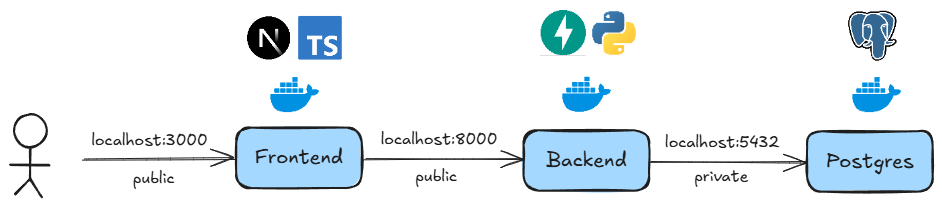
\includegraphics[width=\textwidth]{figures/architecture/main-arch.png}
    \caption{Arquitectura general del proyecto MisiOps}
    \label{fig:main_arch}
\end{figure}

\subsection{Integrantes y roles}
\begin{itemize}
    \item \textbf{Gabriel Espinoza}: Platform Engineer con especialización en Forward Deployment.
    \item \textbf{Jeffrey Monja Castro}: Machine Learning Engineer con especialización en MLOps.
    \item \textbf{Yared Riveros Rodriguez}: DevSecOps Engineer con especialización en hacking.
\end{itemize}


\section{DevSecOps}

\subsection{Importancia de DevSecOps}

MisiOps guarda credenciales de acceso y el historial financiero de cada usuario: ingresos, gastos y presupuestos. Una contraseña filtrada en el repositorio, una dependencia con una vulnerabilidad crítica o una cabecera de seguridad ausente bastan para exponer esos datos y destruir la confianza en el producto. En un esquema tradicional la seguridad se revisa al final, cuando corregir es caro y el código vulnerable ya está publicado.

DevSecOps integra los controles de seguridad dentro del mismo flujo de entrega continua (\textit{shift-left}): cada cambio se analiza automáticamente en el pipeline, los hallazgos se centralizan en un único lugar con historial y ningún cambio con una alerta abierta llega a la rama de producción. En MisiOps esto se traduce en tres decisiones concretas:

\begin{itemize}
    \item \textbf{Seguridad automatizada en cada PR}: SAST, DAST, escaneo de secretos, SCA con SBOM, escaneo de imágenes y de configuración corren en GitHub Actions con versiones fijadas de cada herramienta.
    \item \textbf{Centralización}: los 11 reportes de cada corrida se importan en DefectDojo, donde se triagean, se marcan falsos positivos y se aceptan riesgos con fecha de vencimiento.
    \item \textbf{Gates}: en \texttt{main} los hallazgos bloqueantes impiden el merge; en \texttt{develop} el mismo análisis solo reporta, mediante la exención temporal EX-001 de la constitución del proyecto (vigente hasta el 2026-12-31).
\end{itemize}

La parte de seguridad se desarrolló con el mismo flujo SDD del proyecto: especificación, evaluación, plan, checklist de seguridad y tareas en \texttt{specs/011-devsecops/}, integradas mediante el PR \#130 y el PR \#132 hacia \texttt{develop}.

\subsection{Modelado de amenazas STRIDE}

El modelo de amenazas se construyó como un diagrama de flujo de datos de MisiOps con sus límites de confianza: Internet, la red Docker \texttt{public} (frontend y backend), la red Docker \texttt{private} (PostgreSQL), GitHub (repositorio y CI) y el equipo local donde corre DefectDojo con el túnel ngrok. Cada amenaza se marca sobre el componente o flujo afectado con su letra STRIDE y su identificador (Figura~\ref{fig:stride}).

\begin{figure}[H]
    \centering
    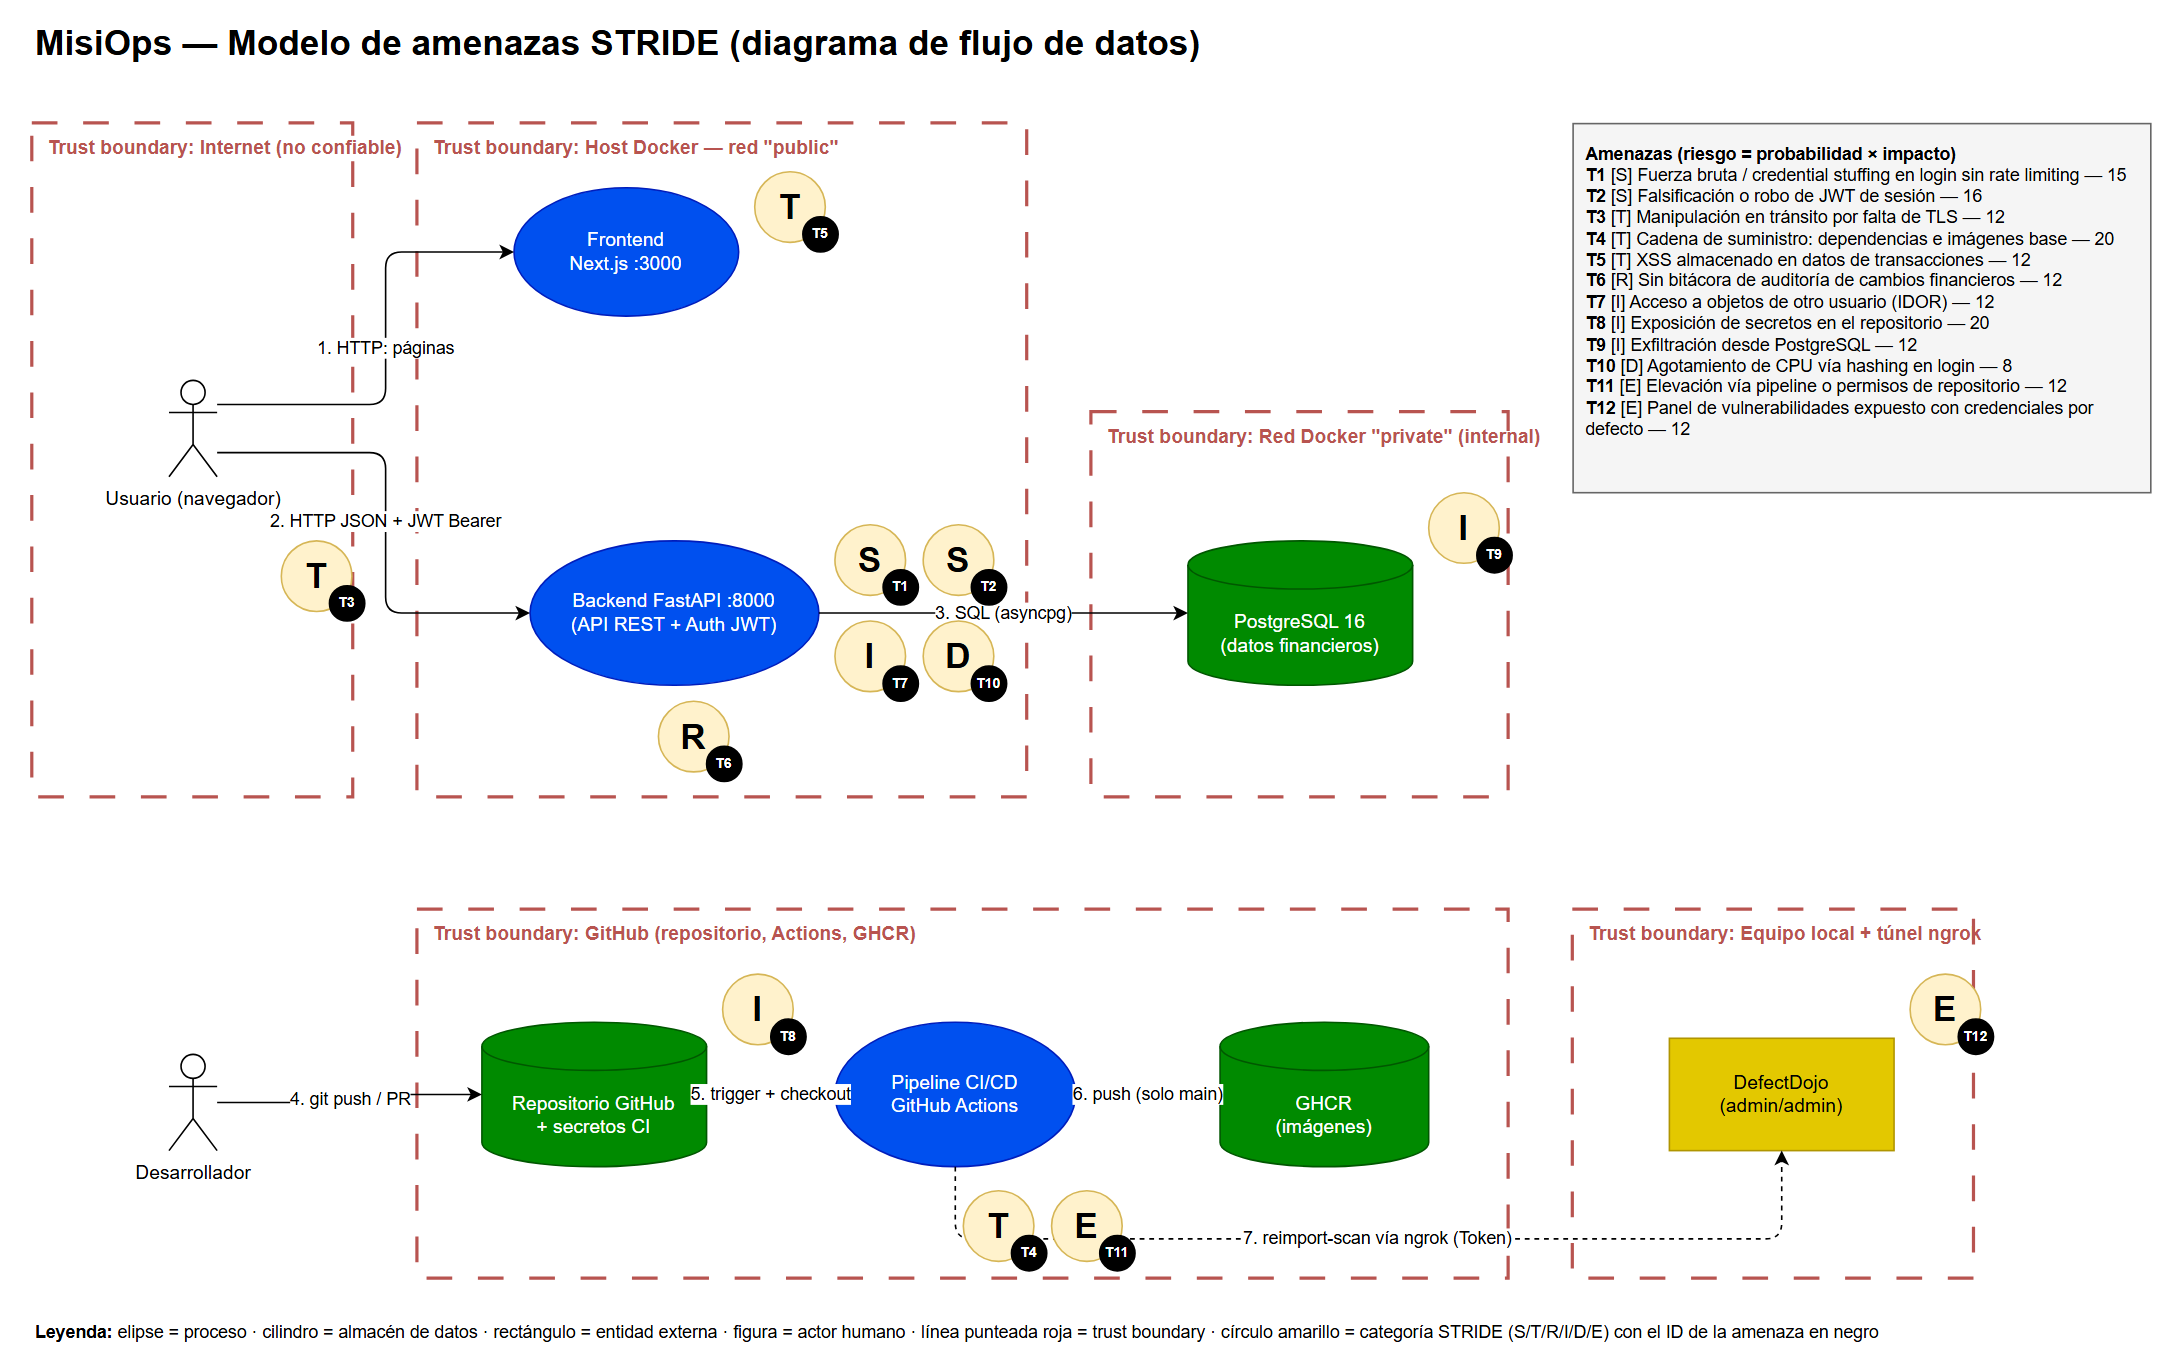
\includegraphics[width=\textwidth]{figures/devsecops/misiops-stride.png}
    \caption{Diagrama STRIDE de MisiOps con límites de confianza e identificadores de amenazas}
    \label{fig:stride}
\end{figure}

La plantilla STRIDE del curso se completó con 12 amenazas que cubren las seis categorías. Para cada una se registró probabilidad e impacto (OWASP Risk Rating, escala 1--5), riesgo inherente, controles actuales, efectividad y riesgo residual.

\begin{itemize}
    \item Diagrama editable (draw.io): \url{https://drive.google.com/file/d/1KUr076G14cM2zBuOgaE54n6_bmTbzVqY/view?usp=sharing}
    \item Plantilla STRIDE: \url{https://docs.google.com/spreadsheets/d/1e4LJ7QdhE3OWo3MIgwexaNvFtrVSTK0w/edit?usp=sharing}
    \item En el repositorio: \texttt{docs/devsecops/stride/} (\texttt{.drawio}, \texttt{.png}, \texttt{.xlsx} y \texttt{amenazas.json}).
\end{itemize}

\subsubsection{Cinco principales vulnerabilidades}

Las amenazas se ordenaron por riesgo $=$ probabilidad $\times$ impacto. En caso de empate se prioriza la que afecta credenciales o datos financieros. La Tabla~\ref{tab:stride-top5} resume las cinco principales.

\begin{table}[H]
    \centering
    \small
    \caption{Cinco amenazas STRIDE priorizadas}
    \label{tab:stride-top5}
    \begin{tabularx}{\textwidth}{@{}c l X c c X@{}}
        \toprule
        \textbf{\#} & \textbf{ID} & \textbf{Amenaza} & \textbf{STRIDE} & \textbf{P$\times$I} & \textbf{Mitigación} \\
        \midrule
        1 & T8 & Un secreto (\texttt{SECRET\_KEY}, contraseña de BD, token de DefectDojo) se sube al repositorio público o queda en el historial & I & 20 & Gitleaks y TruffleHog sobre todo el historial en CI, hook pre-commit, secretos solo en GitHub Secrets \\
        2 & T4 & Una dependencia vulnerable o una imagen base sin versión fija entra a la imagen publicada & T & 20 & SCA, SBOM y escaneo de imágenes con Trivy; \texttt{uv} fijado por digest; entrega solo si todo pasa \\
        3 & T2 & Falsificar o reutilizar un JWT si la \texttt{SECRET\_KEY} es débil o se filtra & S & 16 & Clave de al menos 32 bytes desde secretos; propuesto: rotación y revocación \\
        4 & T1 & Fuerza bruta o \textit{credential stuffing} en \texttt{/auth/login}, sin límite de intentos & S & 15 & argon2 y respuesta uniforme; propuesto: \textit{rate limiting} y bloqueo temporal \\
        5 & T7 & IDOR: cambiar el ID en \texttt{/transactions/\{id\}} para ver datos de otro usuario & I & 12 & Cada consulta filtra por el \texttt{user\_id} del token, con tests de 404 para recursos ajenos \\
        \bottomrule
    \end{tabularx}
\end{table}

\begin{enumerate}
    \item \textbf{T8 -- Fuga de secretos (Information Disclosure).} El repositorio es público y el historial de Git es permanente: un secreto subido una sola vez queda accesible aunque luego se borre. Con la \texttt{SECRET\_KEY} un atacante firma tokens válidos; con la contraseña de la base de datos accede a todos los datos financieros. Por eso el pipeline escanea todo el historial con dos detectores independientes y el hook local bloquea el commit antes de que llegue al remoto.
    \item \textbf{T4 -- Cadena de suministro (Tampering).} Las imágenes del backend y del frontend incluyen cientos de paquetes de terceros. Una versión vulnerable o una imagen base sin versión fija (\texttt{uv:latest}) puede cambiar entre dos builds sin que nadie lo note. El pipeline genera un SBOM, escanea dependencias e imágenes y publica exactamente las imágenes que fueron escaneadas.
    \item \textbf{T2 -- Suplantación con JWT (Spoofing).} La sesión depende de un JWT firmado con HS256. Si la clave es débil o se filtra, cualquiera puede emitir un token para otro usuario. La clave se genera con al menos 32 bytes y se inyecta como secreto; queda pendiente la rotación y revocación de tokens.
    \item \textbf{T1 -- Fuerza bruta en el login (Spoofing).} El endpoint de login no limita intentos. Las contraseñas se guardan con argon2 y la respuesta es uniforme para no revelar si el correo existe, pero falta \textit{rate limiting}, que queda como recomendación.
    \item \textbf{T7 -- IDOR (Information Disclosure).} Los recursos se identifican por ID. Si el backend no comprobara el dueño, bastaría cambiar el número en la URL para leer transacciones ajenas. Todas las consultas filtran por el usuario del token y existen tests que esperan 404 para recursos de otro usuario.
\end{enumerate}

T8 y T4 fueron las que más guiaron el diseño del pipeline: los escáneres de secretos y de dependencias e imágenes existen precisamente para cerrarlas.

\subsection{Análisis estático y dinámico (SAST y DAST)}

\subsubsection{Estrategias}

\begin{itemize}
    \item \textbf{SAST} (\textit{Static Application Security Testing}) analiza el código fuente sin ejecutarlo y busca patrones inseguros: inyección, uso de funciones peligrosas, criptografía débil o secretos en el código. Se ejecuta temprano y es barato, pero no ve cómo se comporta la aplicación desplegada.
    \item \textbf{DAST} (\textit{Dynamic Application Security Testing}) ataca la aplicación en ejecución desde afuera, como lo haría un atacante: revisa cabeceras, cookies, respuestas de error y la superficie de la API. Complementa al SAST porque detecta problemas de configuración que no están en el código.
\end{itemize}

\begin{table}[H]
    \centering
    \small
    \caption{Herramientas de SAST y DAST}
    \begin{tabularx}{\textwidth}{@{}l p{4.2cm} X@{}}
        \toprule
        \textbf{Tipo} & \textbf{Herramienta} & \textbf{Motivo de la elección} \\
        \midrule
        SAST & Semgrep 1.183.0 (\texttt{p/default}, \texttt{p/python}, \texttt{p/typescript}) & Cubre Python y TypeScript con una sola herramienta, tarda menos de 30 s y es la usada en el laboratorio del curso \\
        DAST & OWASP ZAP 2.17.0 (\textit{baseline} y \textit{API scan}) & El \textit{API scan} importa todos los endpoints desde \texttt{/openapi.json} y se autentica con un JWT real, así que también prueba las rutas protegidas \\
        \bottomrule
    \end{tabularx}
\end{table}

\subsubsection{Implementación y evidencia}

Ambos análisis son jobs del workflow \texttt{.github/workflows/devsecops.yml} (Anexo~\ref{anx:devsecops}):

\begin{itemize}
    \item \textbf{Job \texttt{sast}}: ejecuta Semgrep desde su imagen fijada y genera el reporte en JSON y texto. El archivo \texttt{.semgrepignore} excluye reportes archivados y dependencias.
    \item \textbf{Job \texttt{dast}}: levanta el \texttt{docker compose} del proyecto \textbf{con las mismas imágenes que luego se escanean y publican}. Las credenciales de la base de datos y la \texttt{SECRET\_KEY} se generan al vuelo y nunca se versionan. Después registra un usuario temporal, obtiene su token (enmascarado en el log) y corre dos escaneos ZAP: \textit{baseline} sobre el frontend y \textit{API scan} autenticado sobre el backend. Si ZAP no alcanza la aplicación, el job falla en lugar de reportar ``sin hallazgos''.
\end{itemize}

\begin{figure}[H]
    \centering
    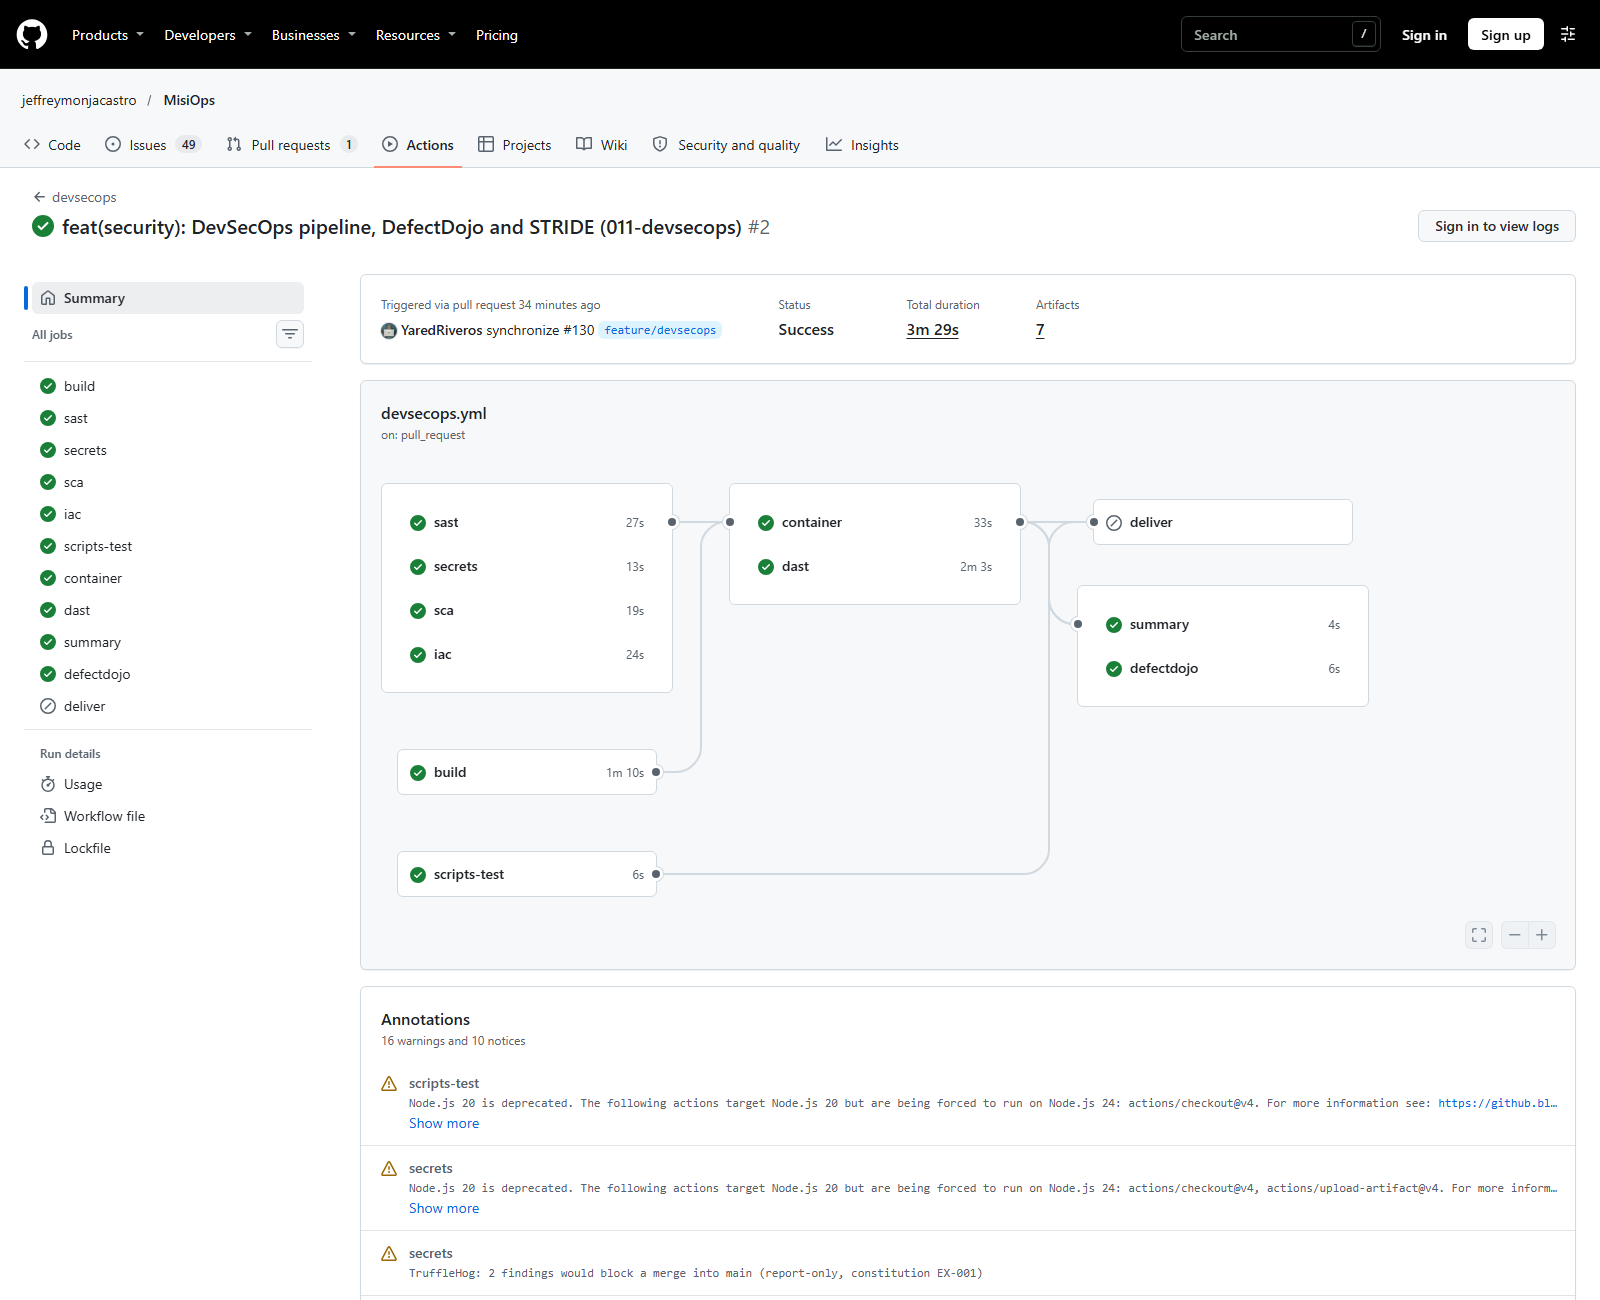
\includegraphics[width=\textwidth]{figures/devsecops/gh-actions-run.png}
    \caption{Corrida del workflow \texttt{devsecops} con los jobs de SAST, DAST y demás escaneos}
    \label{fig:gh-run}
\end{figure}

\subsubsection{Reportes generados}

En la línea base, Semgrep reportó 0 hallazgos en 76 archivos. ZAP reportó 12 alertas en el frontend (Content-Security-Policy ausente, anti-clickjacking, \texttt{X-Content-Type-Options}, \texttt{X-Powered-By}, \texttt{Permissions-Policy}, COOP/CORP) y 6 en la API. Cada corrida guarda los reportes como artefactos durante 7 días, y los de la línea base y del re-escaneo quedaron archivados en \texttt{docs/devsecops/reports/}.

\begin{figure}[H]
    \centering
    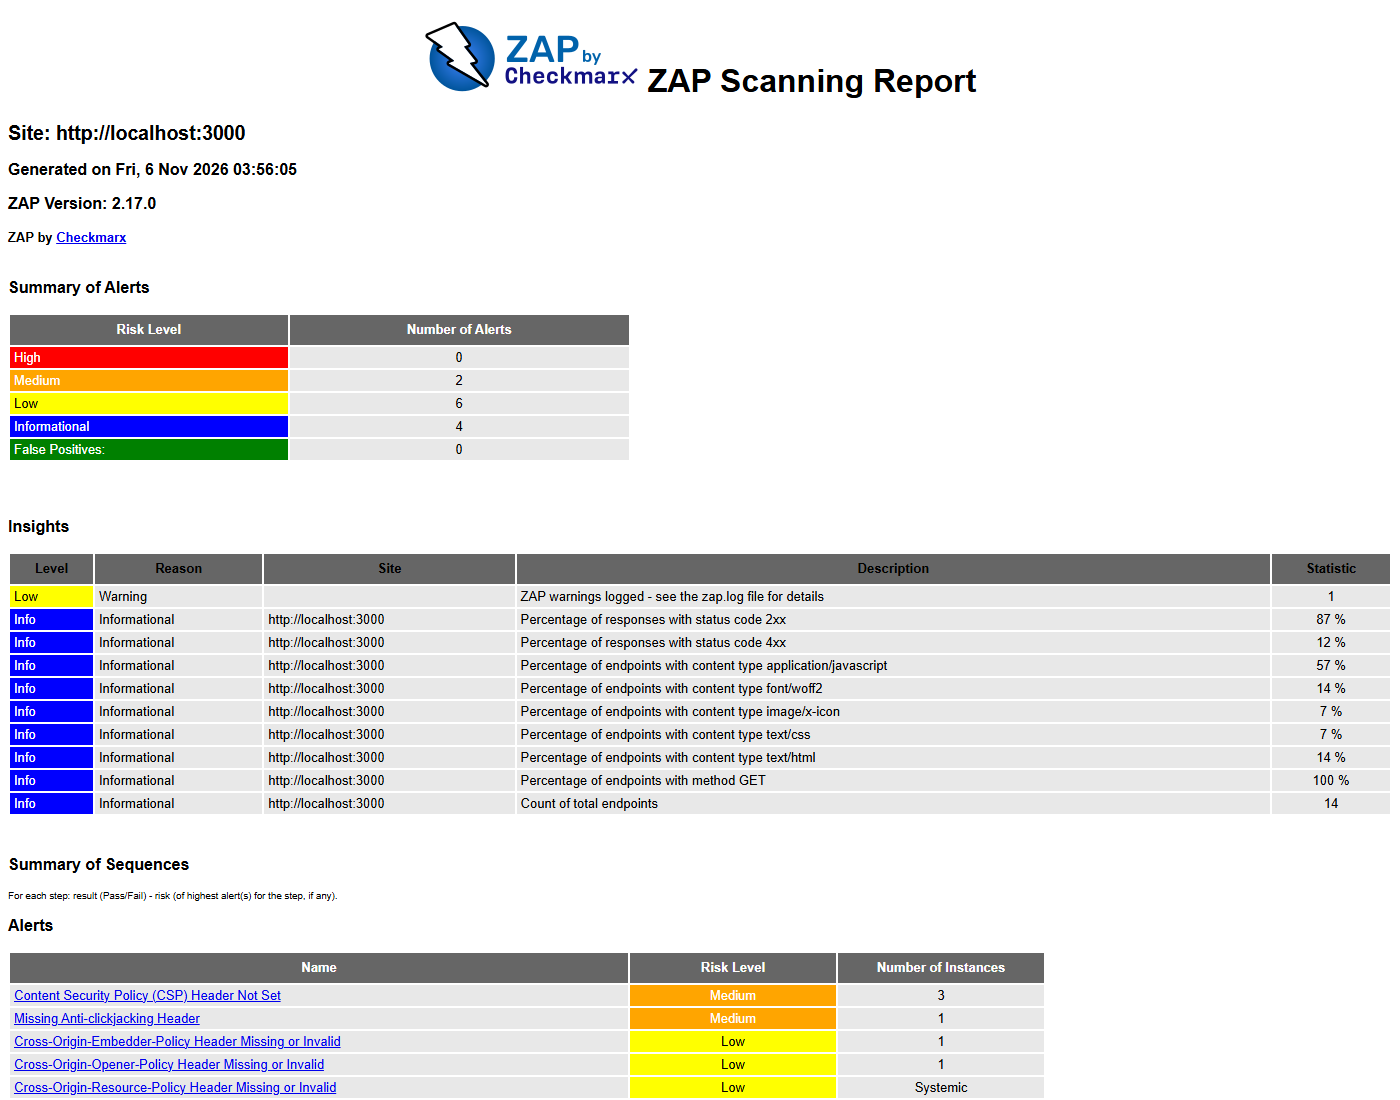
\includegraphics[width=0.9\textwidth]{figures/devsecops/zap-baseline-frontend.png}
    \caption{Reporte HTML de OWASP ZAP sobre el frontend (línea base)}
    \label{fig:zap}
\end{figure}

\subsection{Secret scanning y SCA}

\subsubsection{Estrategias}

\begin{itemize}
    \item \textbf{Secret scanning} busca credenciales (claves de API, tokens, llaves privadas, contraseñas) en el código y en todo el historial de Git, por patrones conocidos y por entropía. Lo ideal es detectarlas antes del commit, porque una vez publicadas hay que rotarlas.
    \item \textbf{SCA} (\textit{Software Composition Analysis}) inventaría las dependencias de terceros, genera un SBOM y las compara con bases de vulnerabilidades conocidas (CVE, GHSA). Se extiende a las imágenes de contenedor, que traen paquetes del sistema operativo, y a la configuración (Dockerfiles y Compose).
\end{itemize}

\begin{table}[H]
    \centering
    \small
    \caption{Herramientas de secretos, SCA, imágenes y configuración}
    \begin{tabularx}{\textwidth}{@{}p{2.4cm} p{4.2cm} X@{}}
        \toprule
        \textbf{Tipo} & \textbf{Herramienta} & \textbf{Alcance} \\
        \midrule
        Secretos (CI) & Gitleaks 8.30.1 & Patrones y entropía sobre todo el historial (\texttt{fetch-depth: 0}) \\
        Secretos (CI) & TruffleHog 3.99.8 & Segundo detector independiente sobre el historial, con verificación de credenciales vivas \\
        Secretos (local) & pre-commit (Gitleaks y \texttt{detect-private-key}) & Bloquea el commit antes de que llegue al repositorio \\
        SCA y SBOM & Trivy 0.76.1 \texttt{fs} & \texttt{backend/uv.lock} y \texttt{frontend/pnpm-lock.yaml}, más un SBOM CycloneDX \\
        Imágenes & Trivy \texttt{image} & Imágenes backend y frontend construidas en el job, más \texttt{postgres} \\
        Configuración & Trivy \texttt{config} y Semgrep \texttt{p/docker-compose} & Dockerfiles y \texttt{docker-compose.yaml} \\
        \bottomrule
    \end{tabularx}
\end{table}

\subsubsection{Implementación y evidencia}

Los jobs \texttt{secrets}, \texttt{sca}, \texttt{container} e \texttt{iac} forman parte del mismo workflow. A nivel local, \texttt{.pre-commit-config.yaml} y \texttt{.githooks/pre-commit} ejecutan Gitleaks sobre lo que está en \textit{staging}. La Figura~\ref{fig:precommit} muestra el hook bloqueando un commit con una clave AWS de prueba.

\begin{figure}[H]
    \centering
    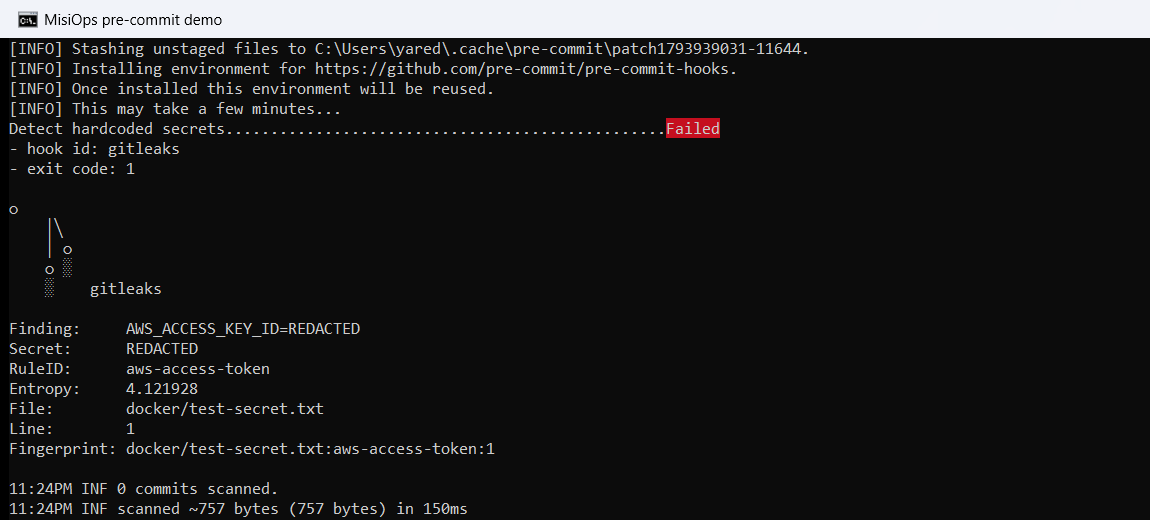
\includegraphics[width=0.9\textwidth]{figures/devsecops/precommit-bloqueo.png}
    \caption{El hook pre-commit bloquea un commit que contiene un secreto}
    \label{fig:precommit}
\end{figure}

\subsubsection{Reportes generados}

\begin{itemize}
    \item \textbf{Secretos}: en la línea base, Gitleaks reportó 4 hallazgos y TruffleHog 2. Tras revisarlos uno por uno, todos eran falsos positivos: nombres de claves de \texttt{localStorage}, la clave AWS de ejemplo del quickstart, un hash de \texttt{uv.lock} y datos de imagen de un diagrama. Quedaron en las listas de excepciones (\texttt{.gitleaks.toml}, \texttt{security/trufflehog-exclude.txt}) con justificación y fecha de revisión.
    \item \textbf{SCA}: Trivy encontró \textbf{7 CRITICAL y 9 HIGH} en las dependencias: Next.js 16.3.4, certifi, dnspython, sharp, source-map-js y un \texttt{package-lock.json} de npm obsoleto que duplicaba hallazgos.
    \item \textbf{Imágenes}: 7 hallazgos bloqueantes en la imagen backend, 64 en la frontend y 170 en \texttt{postgres:16.3}.
\end{itemize}

Los reportes están en \texttt{docs/devsecops/reports/baseline/} (\texttt{trivy-deps.txt}, \texttt{sbom.cdx.json}, \texttt{gitleaks.json}, \texttt{trufflehog.json} y los \texttt{trivy-image-*.json}).

\subsection{DefectDojo}

\subsubsection{Descripción}

DefectDojo es una plataforma open source de gestión de vulnerabilidades (OWASP). Importa los reportes de más de 200 escáneres, los normaliza en hallazgos con severidad, elimina duplicados entre corridas y permite gestionar su ciclo de vida: activo, mitigado, falso positivo o riesgo aceptado. En MisiOps se usa la versión 3.4.202, desplegada en local con Docker Compose, con esta jerarquía:

\begin{center}
    \textit{Product Type} ``Aplicaciones Web'' $\rightarrow$ \textit{Product} ``MisiOps'' $\rightarrow$ \textit{Engagement} ``CI - \textless rama\textgreater'' $\rightarrow$ un \textit{Test} por reporte
\end{center}

\subsubsection{Conexión con GitHub Actions}

\begin{itemize}
    \item DefectDojo corre en un equipo del equipo de trabajo y se expone a GitHub Actions mediante un túnel ngrok con dominio fijo.
    \item El job \texttt{defectdojo} lee los secretos de repositorio \texttt{DEFECTDOJO\_URL} y \texttt{DEFECTDOJO\_TOKEN}. Luego ejecuta \texttt{security/scripts/upload\_to\_defectdojo.sh} (Anexo~\ref{anx:upload}), que sube cada reporte con \texttt{POST /api/v2/reimport-scan/}.
    \item El archivo \texttt{security/scripts/reports.tsv} asocia cada reporte con su parser de DefectDojo y con un título de \textit{Test} propio (por ejemplo ``Trivy - image backend''). Con un título compartido, como en el script del laboratorio, la importación de un reporte cerraba los hallazgos de otro.
    \item La reimportación con \texttt{close\_old\_findings} no duplica hallazgos y marca como mitigados los que ya no aparecen.
    \item Si el túnel no está activo, la subida se omite sin romper los escaneos. Luego \texttt{security/scripts/import\_run.sh \textless run-id\textgreater} descarga los artefactos de esa corrida y los importa desde la máquina local.
    \item El script tiene 37 casos de prueba (\texttt{security/tests/test\_upload\_to\_defectdojo.sh}), que corren en CI en el job \texttt{scripts-test}.
\end{itemize}

En la corrida \href{https://github.com/jeffreymonjacastro/MisiOps/actions/runs/42334876339}{42334876339}, el log del job \texttt{defectdojo} muestra \texttt{ok:} para los 11 reportes.

\subsubsection{Capturas de la aplicación}

\begin{figure}[H]
    \centering
    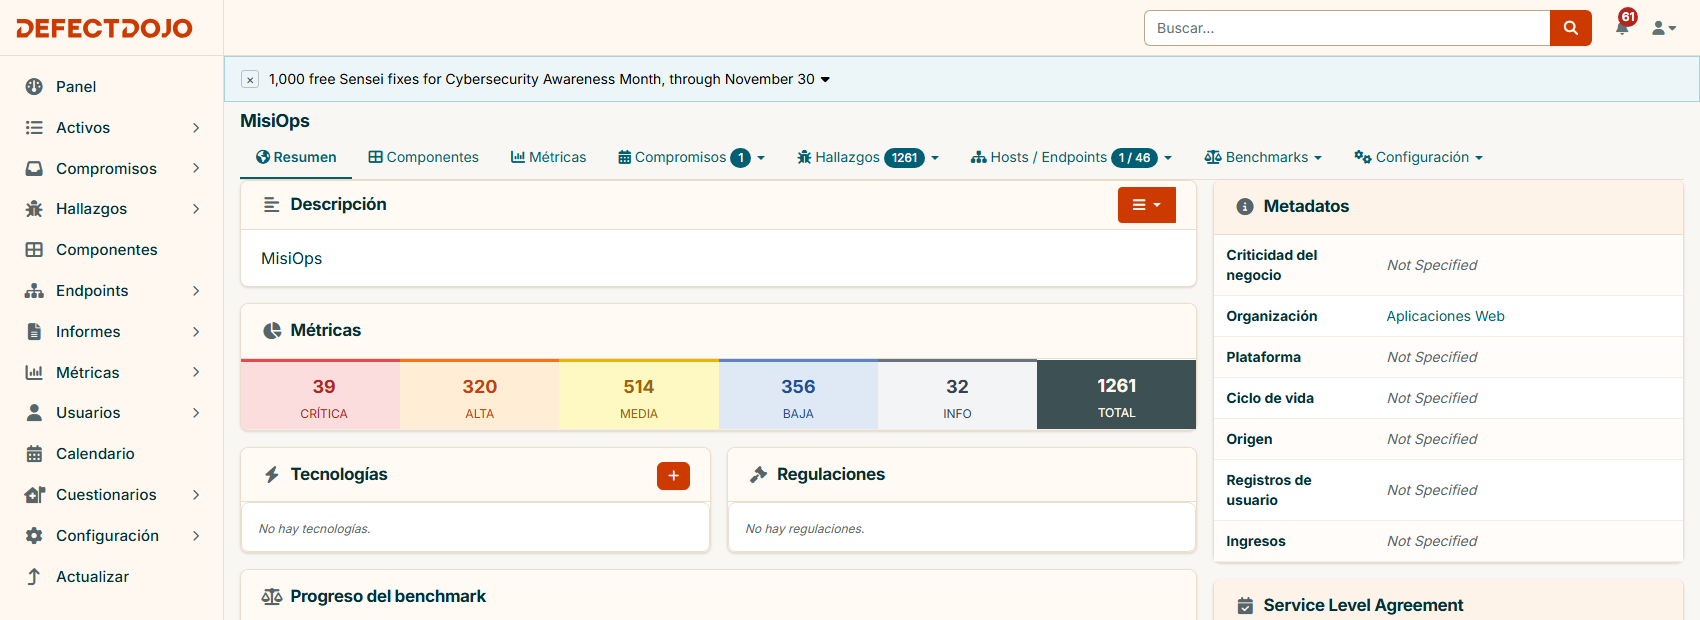
\includegraphics[width=\textwidth]{figures/devsecops/dd-baseline-producto.png}
    \caption{Producto MisiOps en DefectDojo (línea base)}
    \label{fig:dd-producto}
\end{figure}

\begin{figure}[H]
    \centering
    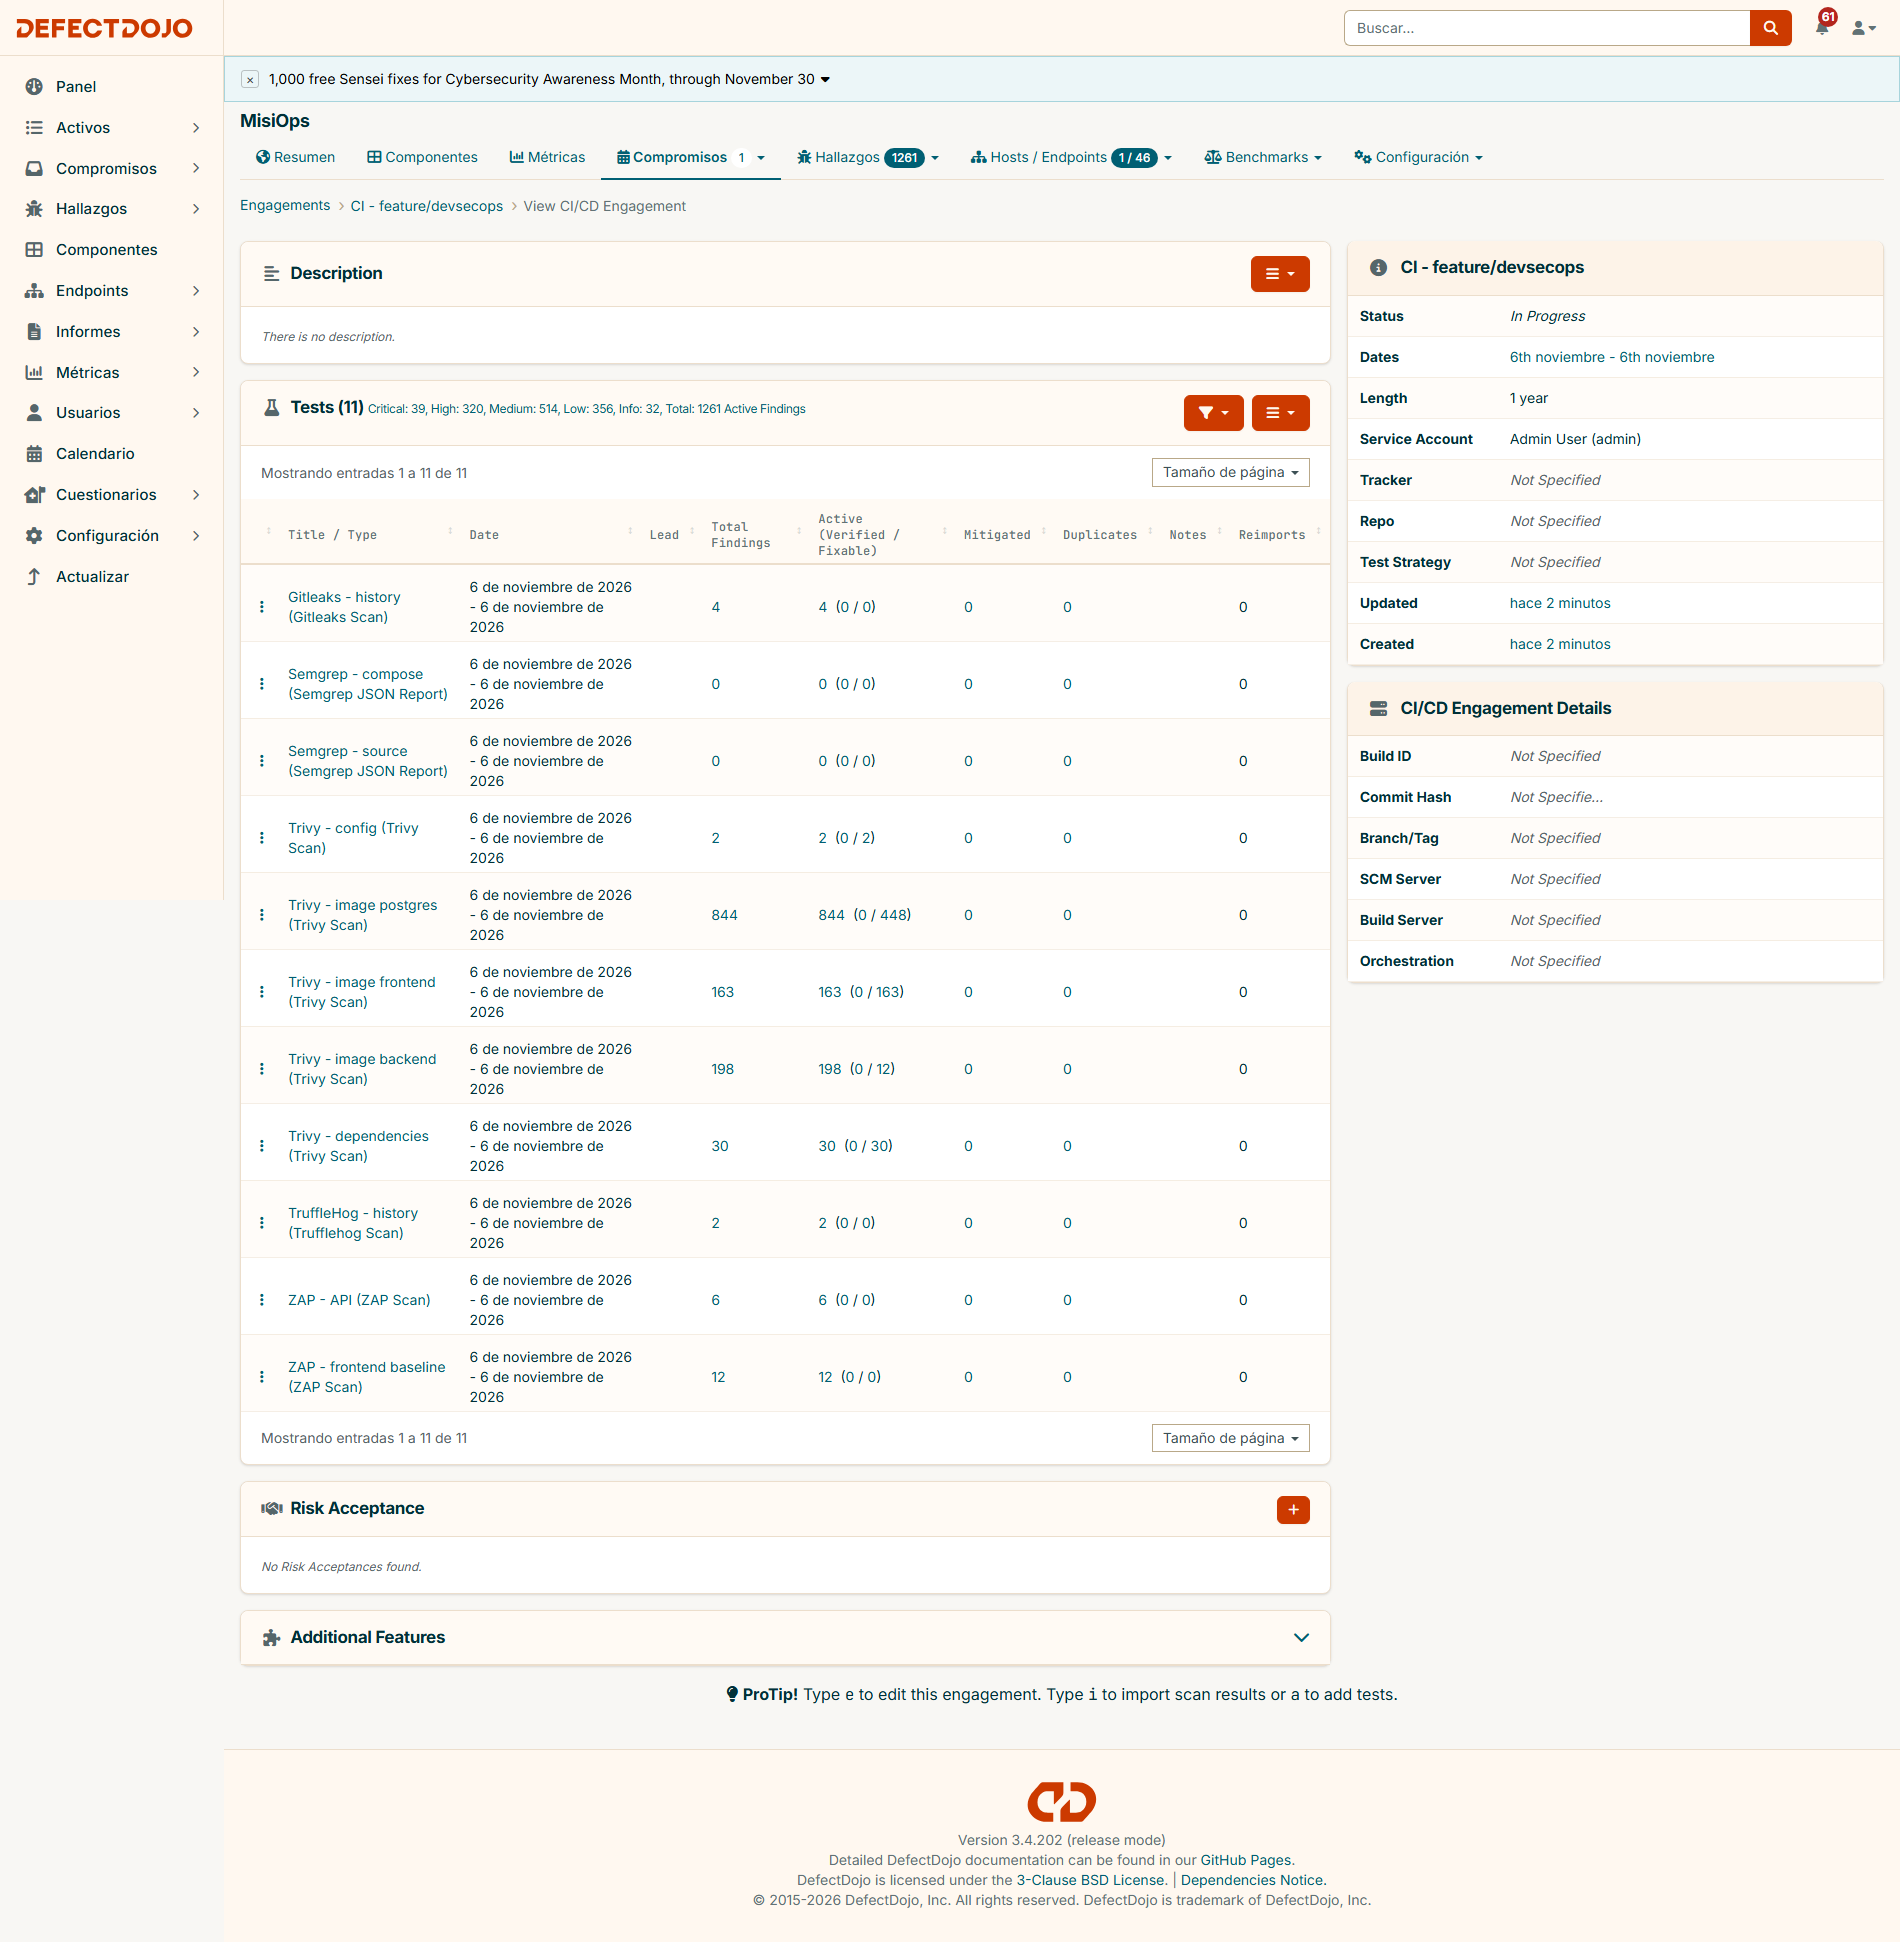
\includegraphics[width=\textwidth]{figures/devsecops/dd-baseline-engagement.png}
    \caption{Engagement de CI con los 11 tests importados (línea base)}
    \label{fig:dd-engagement}
\end{figure}

\begin{figure}[H]
    \centering
    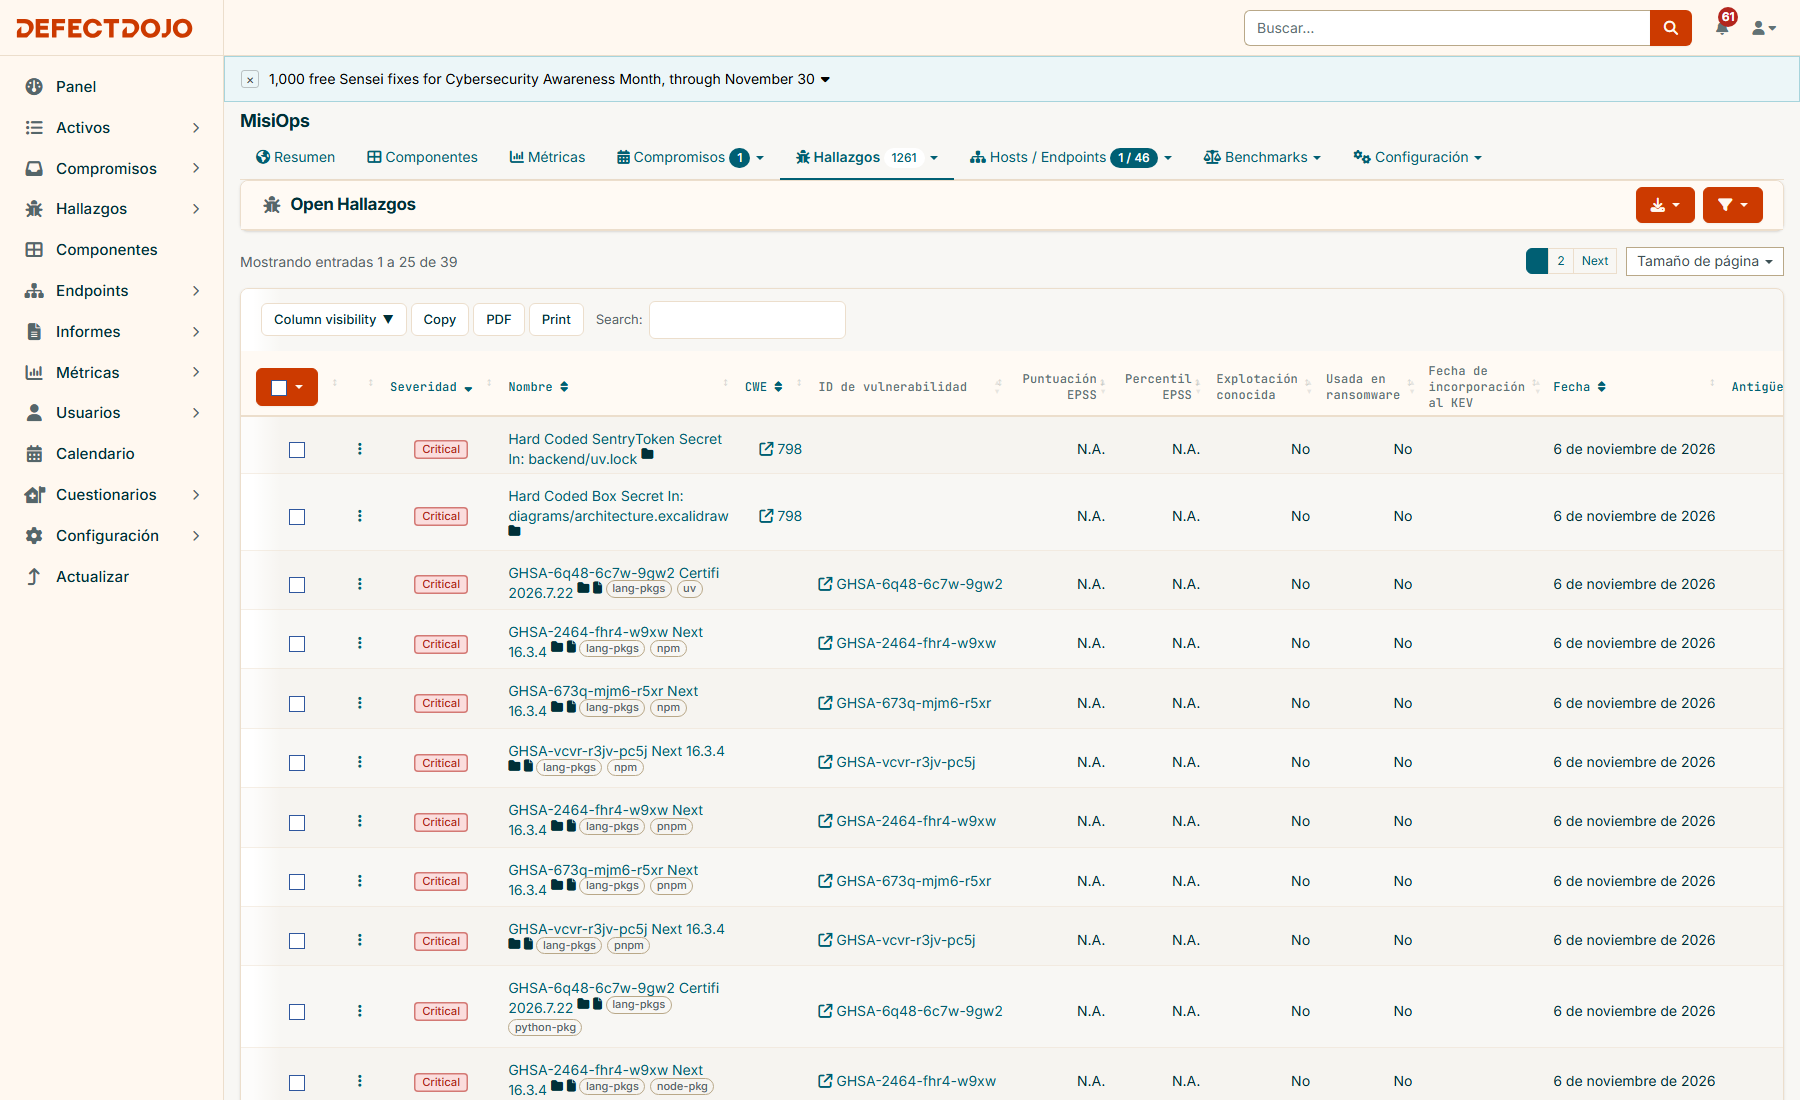
\includegraphics[width=\textwidth]{figures/devsecops/dd-baseline-criticos.png}
    \caption{Hallazgos críticos de la línea base en DefectDojo}
    \label{fig:dd-criticos}
\end{figure}

\subsection{Tabla de mitigaciones}

Los hallazgos se ordenan por severidad. Dentro de una misma severidad, primero va lo que afecta credenciales o datos financieros (amenazas T1, T2, T7, T8 y T9). Cada mitigación cita el commit del PR \#130 que la aplica.

\begin{table}[H]
    \centering
    \scriptsize
    \caption{Hallazgos priorizados y mitigaciones aplicadas}
    \label{tab:mitigaciones}
    \begin{tabularx}{\textwidth}{@{}L{1.25cm} Y L{1.25cm} L{1.65cm} Y L{1.55cm}@{}}
        \toprule
        \textbf{ID} & \textbf{Descripción} & \textbf{Severidad} & \textbf{Herramienta} & \textbf{Mitigación (commit)} & \textbf{Estado} \\
        \midrule
        CRIT-001 & Next.js 16.3.4 con GHSA-vcvr-r3jv-pc5j, GHSA-673q-mjm6-r5xr y GHSA-2464-fhr4-w9xw, en el lockfile y en la imagen frontend & Critical & Trivy SCA e imagen & Subir a \texttt{next} 16.4.5 y eliminar el \texttt{package-lock.json} obsoleto (\texttt{5883661}) & Mitigado \\
        CRIT-002 & certifi 2026.7.22 (GHSA-6q48-6c7w-9gw2), almacén de CA de las conexiones TLS del backend & Critical & Trivy SCA e imagen & Subir a certifi 2026.10.23 (\texttt{5883661}) & Mitigado \\
        CRIT-003 & \texttt{postgres:16.3} con 24 CRITICAL del SO (p.\,ej. libgnutls30 CVE-2026-33845) y 170 hallazgos corregibles & Critical & Trivy imagen & Usar \texttt{postgres:16.15-bookworm} (\texttt{15d7400}) & Mitigado (3 sin fix publicado) \\
        HIGH-001 & PyJWT 2.14.0 (PYSEC-2026-4141, PYSEC-2026-4183), librería de firma de los JWT (T2) & High & pip-audit y Trivy imagen & Subir a pyjwt 2.15.1 (\texttt{fd970da}) & Mitigado \\
        HIGH-002 & \texttt{pip} de la imagen backend trae urllib3, msgpack y setuptools vulnerables & High & Trivy imagen & Desinstalar pip y fijar \texttt{uv} por versión y digest (\texttt{15d7400}) & Mitigado \\
        HIGH-003 & npm y corepack en la imagen frontend (cross-spawn, glob, minimatch) y OpenSSL de Alpine & High & Trivy imagen & Etapa final sin npm ni corepack y con \texttt{apk upgrade} (\texttt{15d7400}) & Mitigado \\
        HIGH-004 & 4 hallazgos de Gitleaks y 2 de TruffleHog en el historial (T8) & High & Gitleaks, TruffleHog & Revisión manual y excepción documentada (\texttt{add48cc}); hook pre-commit & Falso positivo \\
        HIGH-005 & dnspython CVE-2026-114605, sharp GHSA-wq5f-xc86-pv6w, source-map-js CVE-2026-93749 & High & Trivy SCA & Actualizar dependencias directas y transitivas (\texttt{5883661}) & Mitigado \\
        HIGH-006 & 26 CVE de la stdlib de Go en \texttt{gosu} (imagen oficial de postgres) & High & Trivy imagen & \texttt{.trivyignore.yaml} con justificación y vencimiento & Riesgo aceptado \\
        MED-001 & Sin Content-Security-Policy en el frontend (ZAP 10038), habilita XSS (T5) & Medium & ZAP baseline & CSP con \texttt{default-src 'self'} y \texttt{frame-ancestors 'none'} (\texttt{43c0621}) & Mitigado \\
        MED-002 & Sin protección anti-clickjacking (ZAP 10020) & Medium & ZAP baseline & \texttt{X-Frame-Options: DENY} (\texttt{43c0621}) & Mitigado \\
        LOW-001 & Faltan \texttt{X-Content-Type-Options}, \texttt{Permissions-Policy}, COOP/CORP y sobra \texttt{X-Powered-By} & Low & ZAP baseline y API & Cabeceras en \texttt{next.config.ts} y middleware en \texttt{backend/main.py}, con tests (\texttt{43c0621}) & Mitigado \\
        \bottomrule
    \end{tabularx}
\end{table}

\subsection{Técnicas de seguridad y mitigación: antes y después}

\textbf{Antes}, el CI solo tenía lint, tests, build, una prueba de integración con Docker y \texttt{pip-audit}. No había escaneo de secretos, de imágenes ni de configuración, tampoco DAST. Los resultados no se reunían en ningún lugar y nada impedía integrar un cambio inseguro.

\textbf{Después}, cada corrida produce 11 reportes, se centralizan en DefectDojo y un gate impide llegar a \texttt{main} con alertas abiertas. Las técnicas aplicadas fueron:

\begin{itemize}
    \item \textbf{Actualización de dependencias} con fix publicado (Next.js, certifi, PyJWT, dnspython, sharp, source-map-js).
    \item \textbf{Reducción de la superficie de las imágenes}: el backend sin \texttt{pip} y con \texttt{uv} fijado por digest; el frontend sin npm ni corepack; \texttt{postgres} actualizado a una versión parcheada; y \texttt{apt-get upgrade} en la imagen del backend (PR \#180) para que los parches del SO no esperen a la imagen base.
    \item \textbf{Cabeceras de seguridad HTTP} en frontend y backend (CSP, anti-clickjacking, \texttt{nosniff}, \texttt{Permissions-Policy}, COOP/CORP), cubiertas por 7 tests nuevos.
    \item \textbf{Prevención de secretos} desde el commit local y doble detector en CI.
    \item \textbf{Gestión explícita de excepciones}: cada falso positivo o riesgo aceptado vive en el archivo de excepciones de su herramienta, con justificación y fecha de revisión, y se refleja en DefectDojo como \textit{False Positive} o \textit{Risk Acceptance}.
\end{itemize}

La línea base es la corrida \href{https://github.com/jeffreymonjacastro/MisiOps/actions/runs/42159225729}{42159225729} (commit \texttt{ff7ba32}) y el re-escaneo es la corrida \href{https://github.com/jeffreymonjacastro/MisiOps/actions/runs/42162904886}{42162904886} (commit \texttt{a628e9d}), ambas con las mismas versiones y reglas.

\begin{table}[H]
    \centering
    \small
    \caption{Hallazgos activos en DefectDojo antes y después de remediar}
    \label{tab:antes-despues}
    \begin{tabular}{@{}lrrrr@{}}
        \toprule
        \textbf{Severidad} & \textbf{Antes} & \textbf{Después} & \textbf{Cerrados (\textit{Mitigated})} & \textbf{Reducción} \\
        \midrule
        Critical & 39 & 3 & 39 & $-$92\,\% \\
        High & 320 & 93 & 274 & $-$71\,\% \\
        Medium & 514 & 284 & 441 & $-$45\,\% \\
        Low & 356 & 241 & 290 & $-$32\,\% \\
        Info & 32 & 20 & 19 & $-$38\,\% \\
        \midrule
        \textbf{Total} & \textbf{1261} & \textbf{641} & \textbf{1063} & \textbf{$-$49\,\%} \\
        \bottomrule
    \end{tabular}
\end{table}

La columna ``Después'' incluye hallazgos nuevos de las imágenes actualizadas que aún no tienen fix publicado; por eso ``antes menos cerrados'' no coincide exactamente con ``después''. Lo que decide el merge son los hallazgos \textbf{bloqueantes} de cada gate, que bajaron de 263 a 0:

\begin{table}[H]
    \centering
    \small
    \caption{Hallazgos que bloquean el merge a \texttt{main}}
    \begin{tabular}{@{}lrr@{}}
        \toprule
        \textbf{Reporte} & \textbf{Antes} & \textbf{Después} \\
        \midrule
        Trivy dependencias & 16 & 0 \\
        Trivy imagen backend & 7 & 0 \\
        Trivy imagen frontend & 64 & 0 \\
        Trivy imagen postgres & 170 & 0 \\
        Gitleaks y TruffleHog & 6 & 0 \\
        Semgrep, Trivy config y ZAP (High) & 0 & 0 \\
        \midrule
        \textbf{Total} & \textbf{263} & \textbf{0} \\
        \bottomrule
    \end{tabular}
\end{table}

\begin{figure}[H]
    \centering
    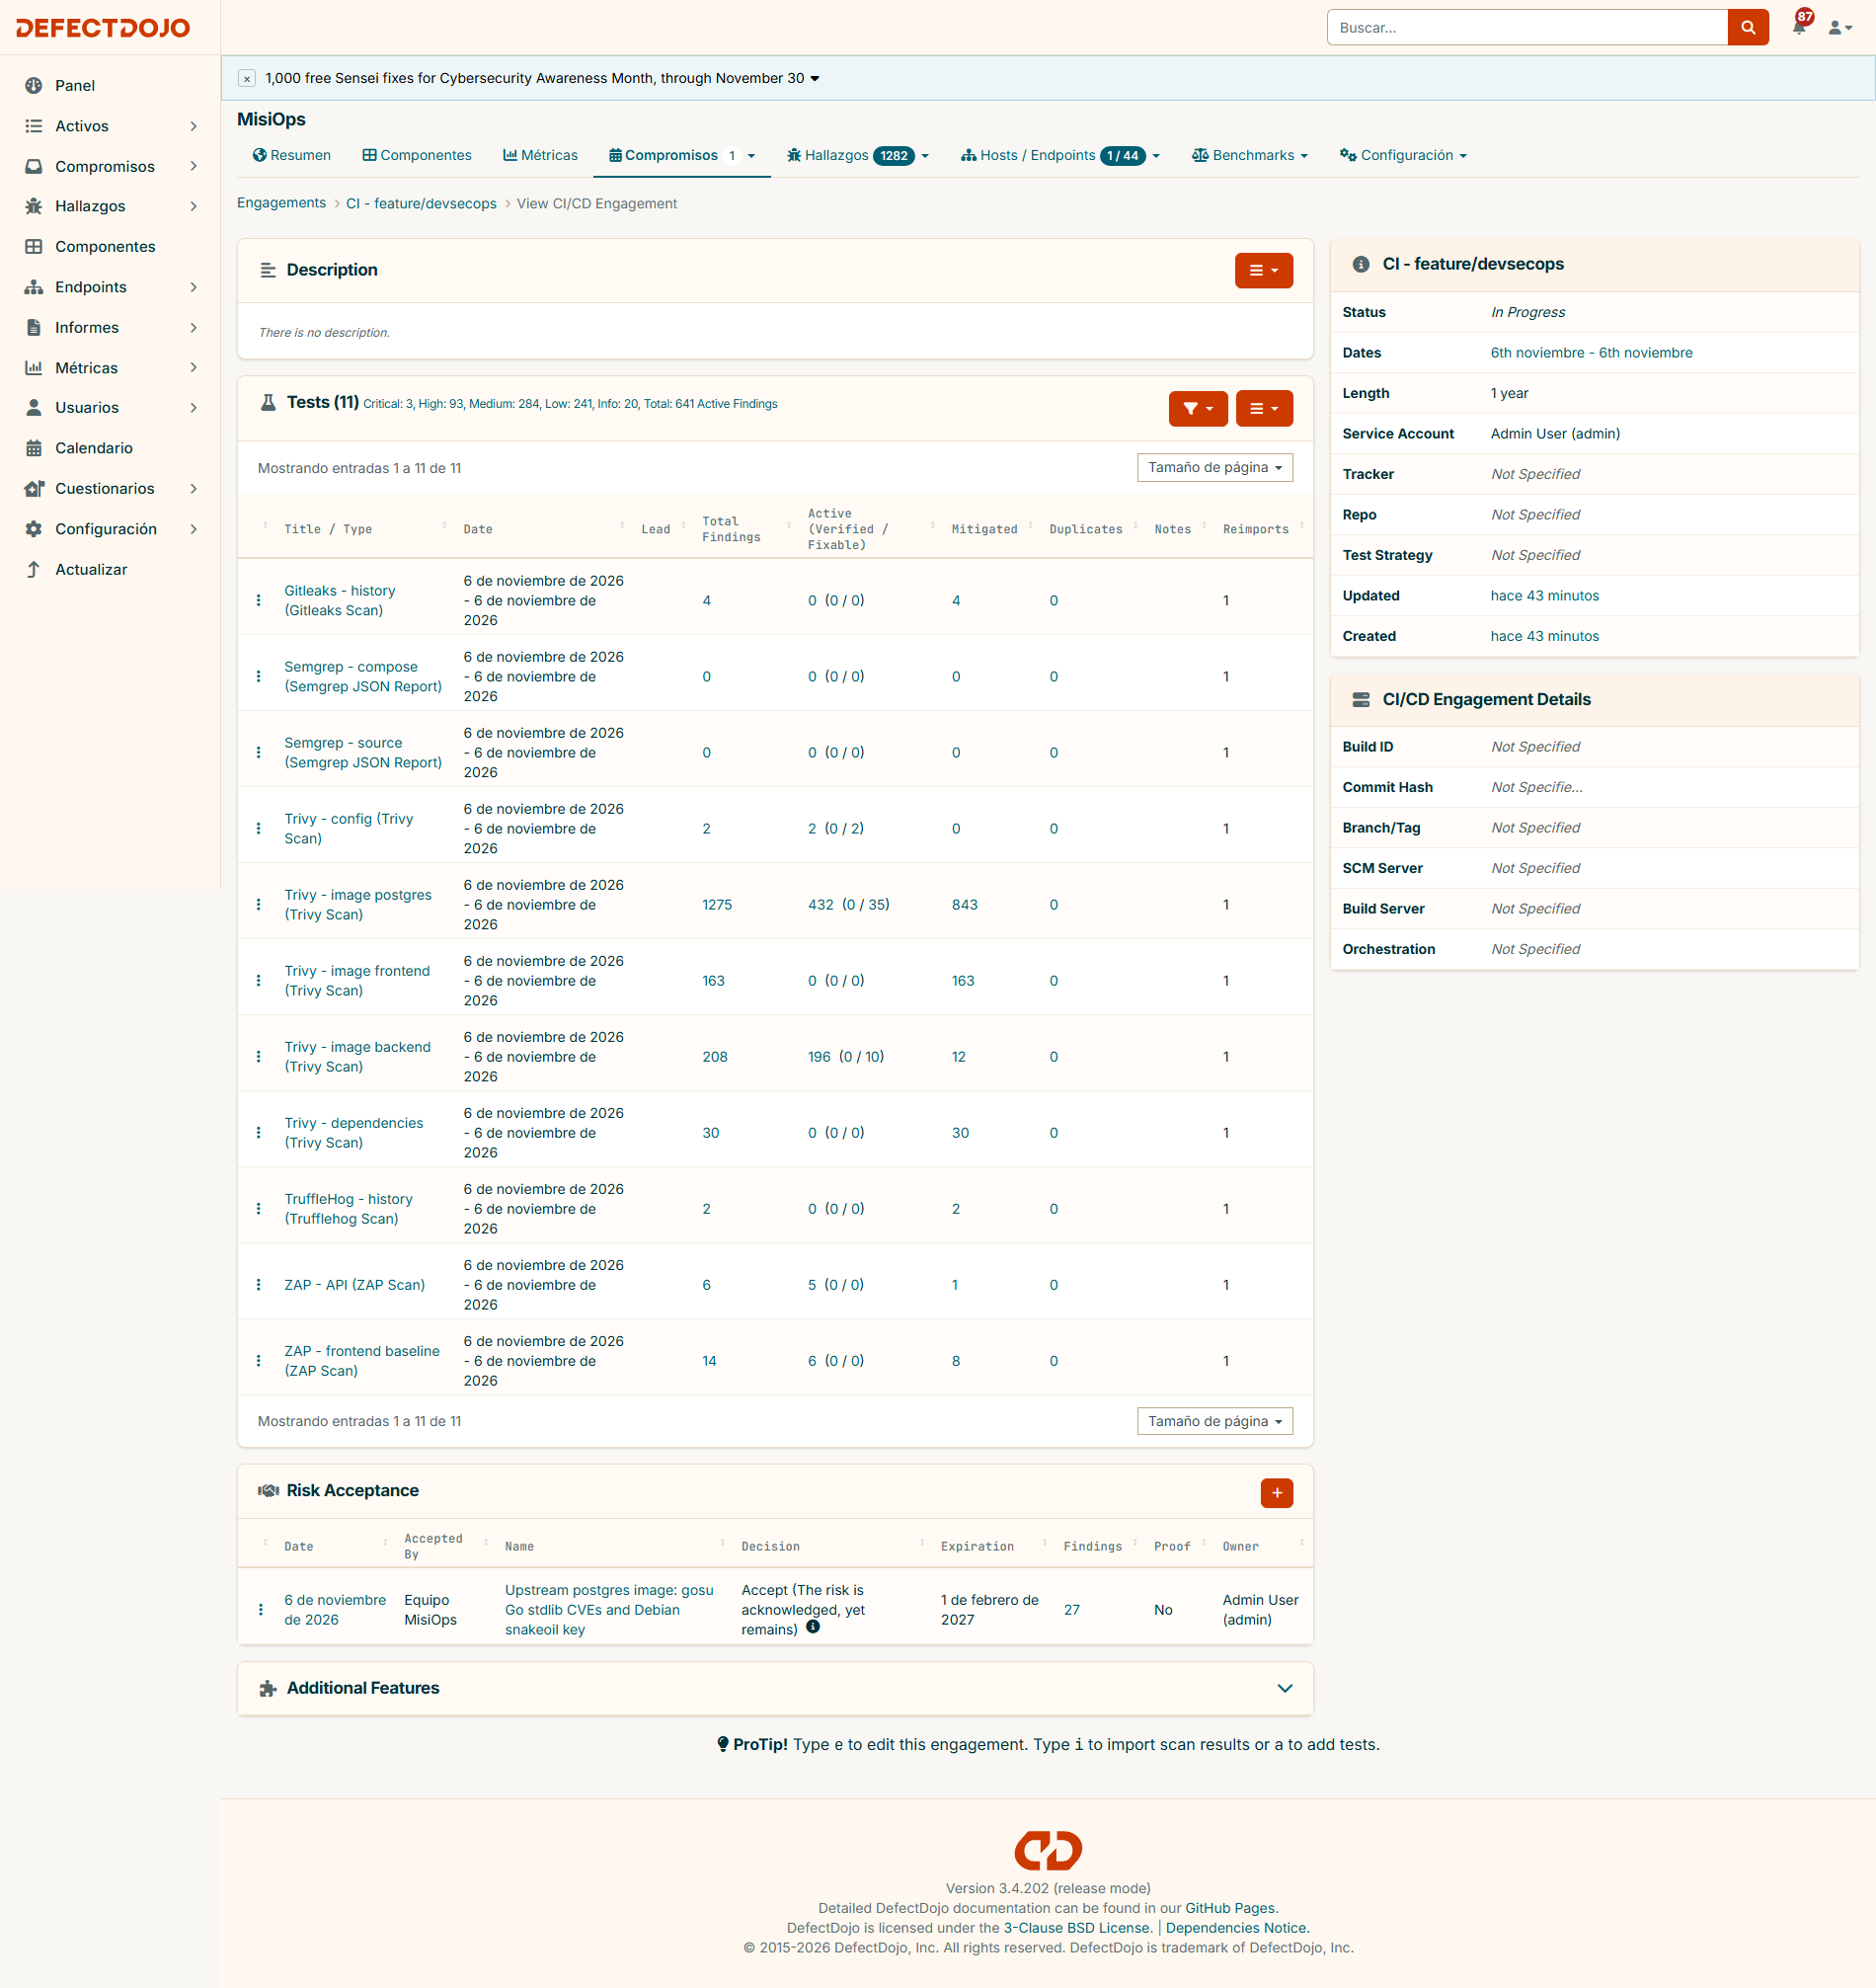
\includegraphics[width=\textwidth]{figures/devsecops/dd-rescan-engagement.png}
    \caption{Engagement después de remediar, con el panel de riesgos aceptados}
    \label{fig:dd-rescan}
\end{figure}

\begin{figure}[H]
    \centering
    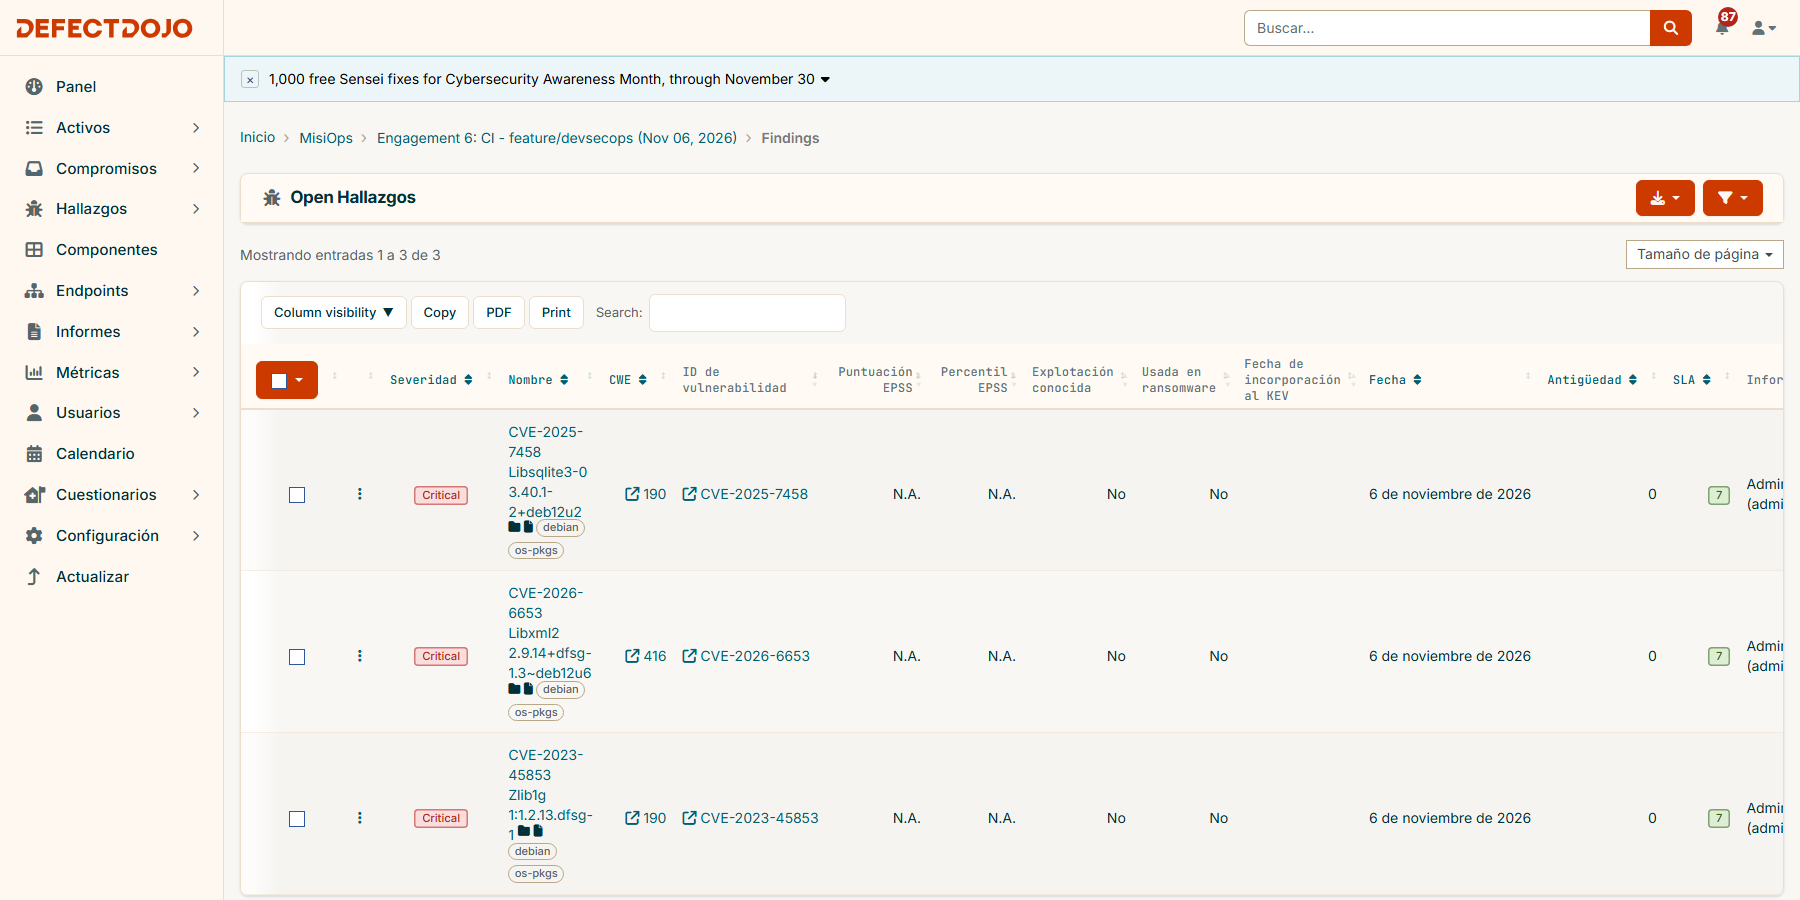
\includegraphics[width=\textwidth]{figures/devsecops/dd-rescan-criticos.png}
    \caption{Críticos abiertos tras el re-escaneo: solo quedan 3 del SO de postgres sin fix publicado}
    \label{fig:dd-rescan-crit}
\end{figure}

Las suites existentes siguen en verde (123 tests del backend y 42 del frontend), igual que lint, build e integración.

\subsection{Pipeline DevSecOps en GitHub Actions}

El workflow \texttt{devsecops.yml} corre en cada PR y en cada push a \texttt{develop} y \texttt{main} (Figura~\ref{fig:pipeline}):

\begin{enumerate}
    \item \textbf{Local}: hook pre-commit (Gitleaks y \texttt{detect-private-key}) y hook pre-push (artefactos SDD).
    \item \textbf{build}: construye una sola vez las imágenes backend y frontend y las guarda como artefacto.
    \item \textbf{En paralelo}: \texttt{sast}, \texttt{secrets}, \texttt{sca}, \texttt{iac} y \texttt{scripts-test}. Cuando termina \texttt{build}, también \texttt{container} (Trivy sobre las 3 imágenes) y \texttt{dast} (ZAP sobre el stack levantado con esas imágenes).
    \item \textbf{Gate por herramienta} (\texttt{security/scripts/gate.sh}): bloquea en \texttt{main} y solo reporta en \texttt{develop}.
    \item \textbf{summary} (tabla en el resumen de la corrida) y \textbf{defectdojo} (reimportación).
    \item \textbf{deliver}: solo en push a \texttt{main} y solo si todos los gates pasaron. Publica en GHCR \textbf{las mismas} imágenes escaneadas.
\end{enumerate}

En paralelo siguen corriendo los workflows de calidad que ya existían: \texttt{backend-ci} (ruff, pytest, pip-audit), \texttt{frontend-ci} (eslint, tests, build), \texttt{docker-integration} y el \texttt{SDD Pipeline Enforcer}. La corrida completa tarda unos 4 minutos.

\begin{figure}[H]
    \centering
    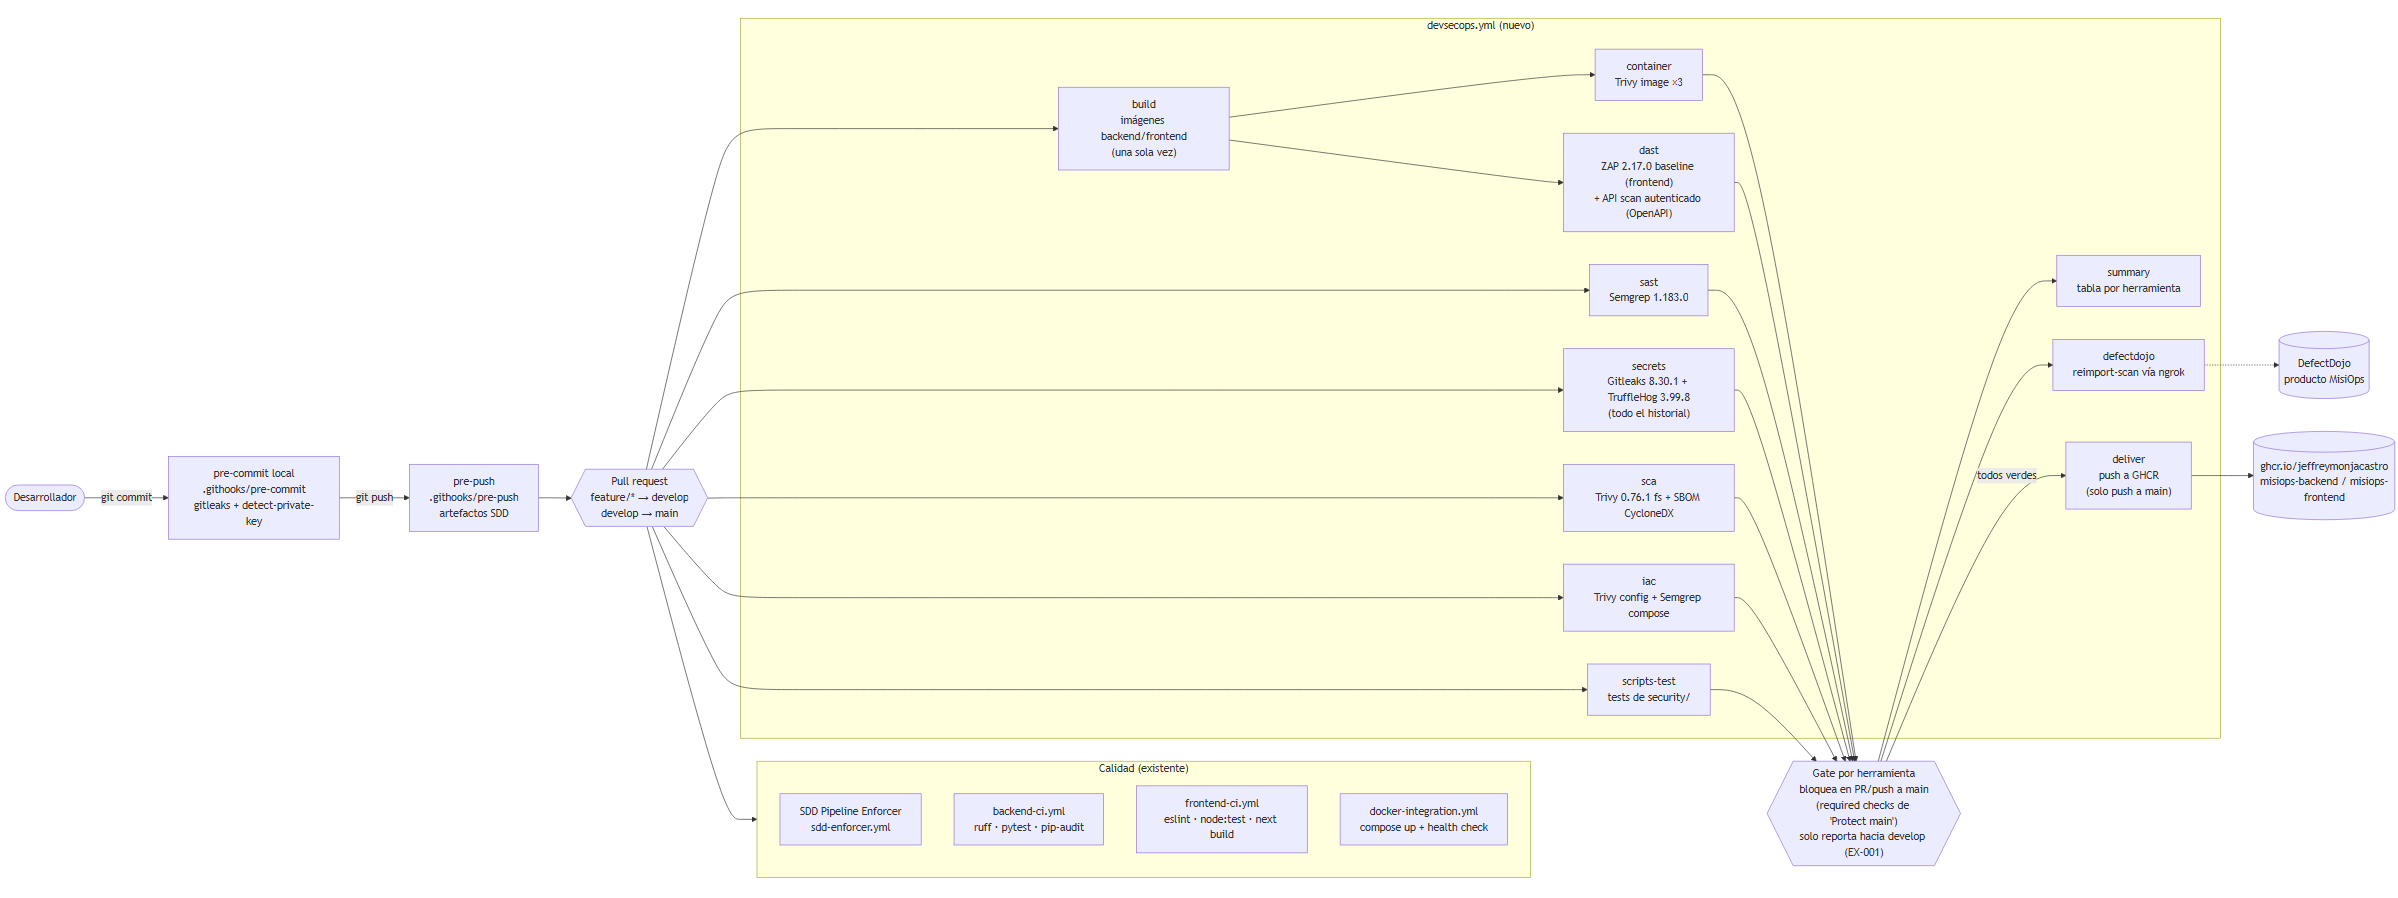
\includegraphics[width=\textwidth]{figures/devsecops/pipeline.png}
    \caption{Diagrama del pipeline CI/CD con las etapas de seguridad}
    \label{fig:pipeline}
\end{figure}

\begin{figure}[H]
    \centering
    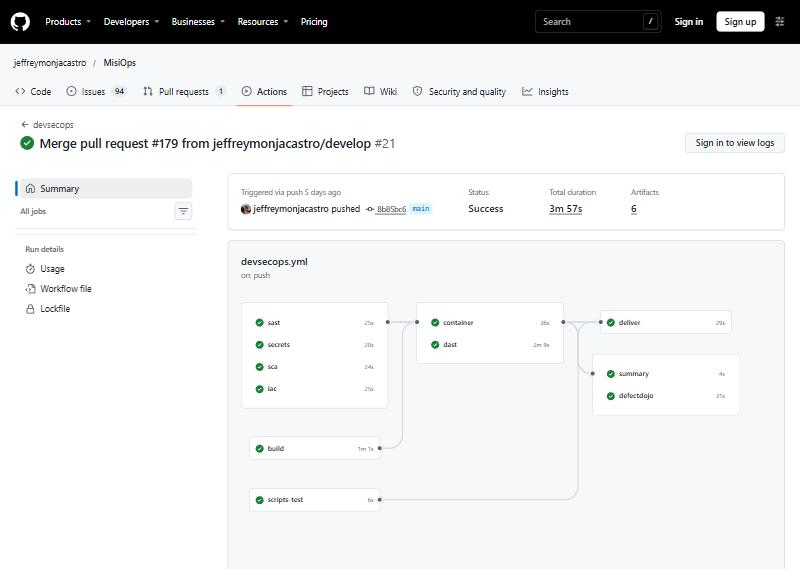
\includegraphics[width=\textwidth]{figures/devsecops/gh-actions-main.jpg}
    \caption{Corrida de \texttt{devsecops} sobre \texttt{main} tras el merge del PR \#179: todos los gates en verde, entrega a GHCR y subida a DefectDojo}
    \label{fig:gh-main}
\end{figure}

\subsubsection{Política de gates}

\begin{table}[H]
    \centering
    \small
    \caption{Condición de bloqueo de cada herramienta}
    \begin{tabularx}{\textwidth}{@{}p{4.5cm} X@{}}
        \toprule
        \textbf{Herramienta} & \textbf{Bloquea cuando...} \\
        \midrule
        Semgrep & Hay algún hallazgo de severidad \texttt{ERROR} \\
        Gitleaks / TruffleHog & Hay cualquier secreto que no esté en la lista de excepciones \\
        Trivy (dependencias e imágenes) & Hay CRITICAL o HIGH \textbf{con versión corregida disponible}; los que no tienen fix solo se reportan \\
        Trivy config / Semgrep compose & Hay alguna mala configuración HIGH o CRITICAL, o un hallazgo \texttt{ERROR} \\
        ZAP & Hay alguna alerta de riesgo High \\
        \bottomrule
    \end{tabularx}
\end{table}

El ruleset ``Protect main'' exige los checks \texttt{sast}, \texttt{secrets}, \texttt{sca}, \texttt{container}, \texttt{iac}, \texttt{dast} y \texttt{scripts-test}, además de una aprobación, y no tiene lista de \textit{bypass}. Para demostrar el bloqueo se abrió el PR de prueba \#131 hacia \texttt{main}: la rama era \texttt{develop} más un Dockerfile que corría como root a propósito (Trivy DS002, HIGH). El gate \texttt{iac} falló con \texttt{Trivy config: 1 blocking findings} y GitHub dejó el merge bloqueado. El PR se cerró sin merge.

\begin{figure}[H]
    \centering
    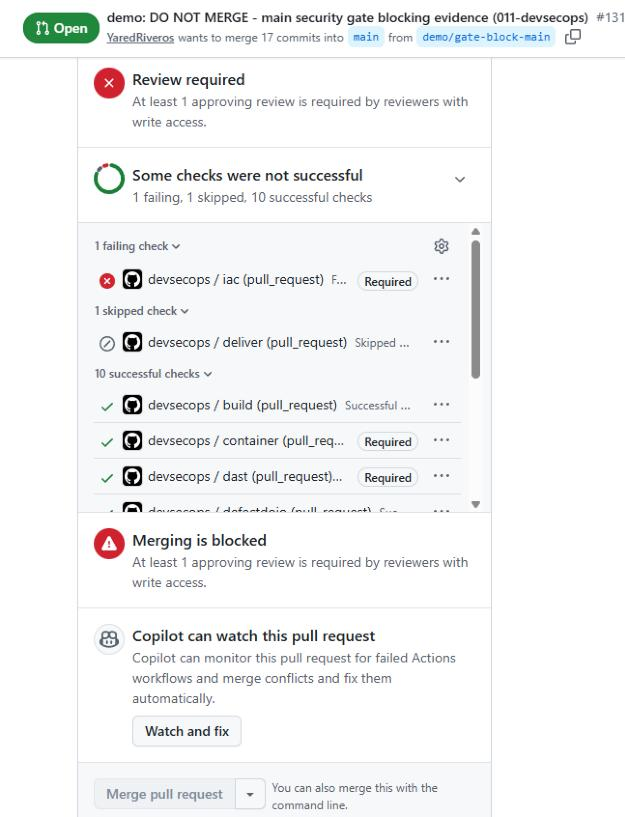
\includegraphics[width=0.85\textwidth]{figures/devsecops/main-merge-bloqueado.png}
    \caption{PR \#131 hacia \texttt{main}: el check requerido \texttt{iac} falla y el botón de merge queda deshabilitado}
    \label{fig:merge-bloqueado}
\end{figure}

\begin{figure}[H]
    \centering
    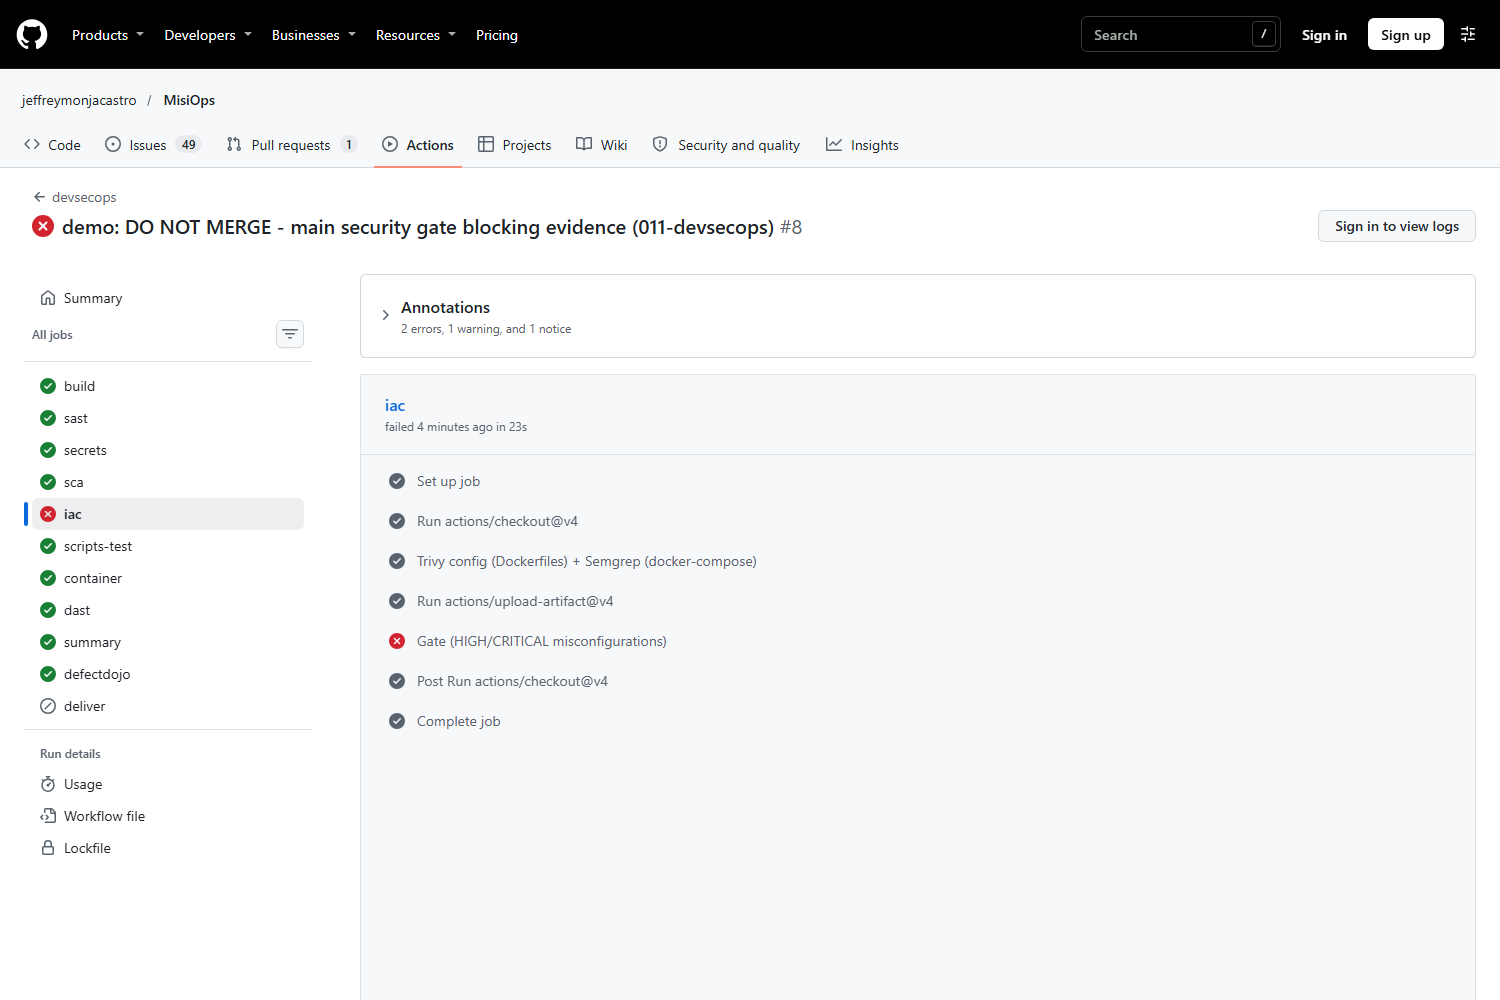
\includegraphics[width=\textwidth]{figures/devsecops/main-gate-iac-falla.png}
    \caption{Corrida del PR \#131: el gate \texttt{iac} detecta el hallazgo bloqueante}
    \label{fig:gate-iac}
\end{figure}

El gate funcionó igual en un caso real: el PR \#179, que promovía \texttt{develop} a \texttt{main}, quedó bloqueado cuando Debian publicó el fix de dos CVE HIGH de \texttt{zlib1g} en la imagen base del backend. Se corrigió con el PR \#180 (\texttt{apt-get upgrade} en el Dockerfile) y la promoción pasó.

Los scripts y archivos de configuración de la parte de seguridad se incluyen en el Anexo~\ref{anx:devsecops-config}.


\section{Infrastructure as Code (IaC)}

\subsection{Importancia de IaC}

Infrastructure as Code consiste en describir la infraestructura (redes, bases de datos, contenedores, permisos) en archivos de código versionados, en lugar de crearla a mano desde la consola del proveedor. Sus ventajas para MisiOps son:

\begin{itemize}
    \item \textbf{Reproducibilidad}: \texttt{dev} y \texttt{prod} salen del mismo código y solo difieren en los parámetros declarados en \texttt{infra/lib/config.ts}. No hay configuración ``invisible'' hecha en la consola.
    \item \textbf{Revisión y trazabilidad}: cada cambio de infraestructura pasa por un PR, por el flujo SDD y por un pipeline de pruebas, igual que el código de la aplicación.
    \item \textbf{Pruebas antes de desplegar}: las propiedades de seguridad (base de datos privada, cifrado, secretos sin texto plano, rol de mínimo privilegio) se verifican con tests automáticos sobre la plantilla generada.
    \item \textbf{Despliegue y rollback automáticos}: CloudFormation aplica los cambios de forma transaccional y revierte si algo falla. Una nueva versión se despliega haciendo merge, sin pasos manuales.
\end{itemize}

La infraestructura se escribió con \textbf{AWS CDK en TypeScript} (\texttt{aws-cdk-lib} 2.273.0). CDK genera (\textit{synth}) plantillas de \textbf{AWS CloudFormation}, y CloudFormation es el servicio que crea, actualiza y revierte los recursos. Esta parte se desarrolló con el flujo SDD en \texttt{specs/012-aws-deployment/} y se integró con el PR \#178.

\subsection{Arquitectura de IaC y componentes}

\begin{figure}[H]
    \centering
    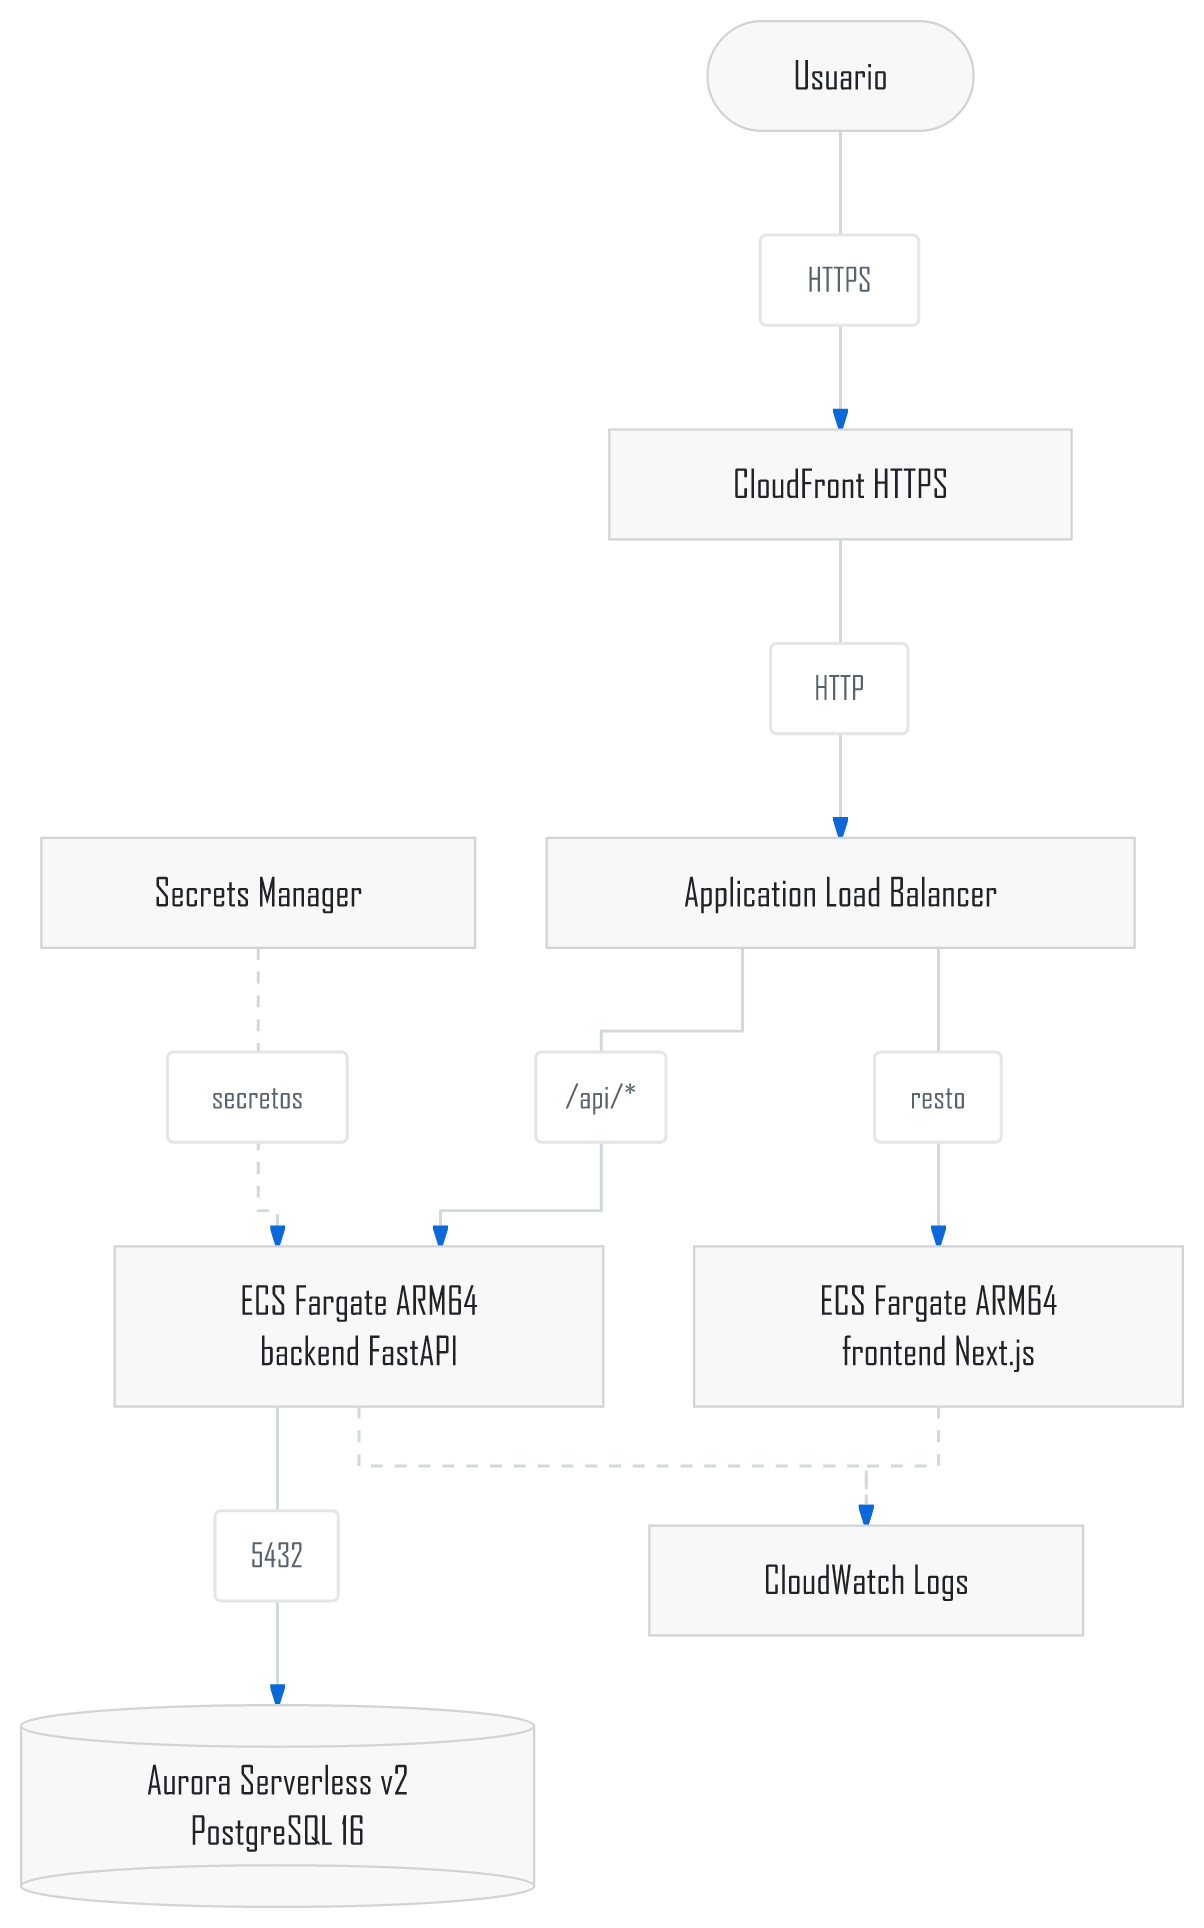
\includegraphics[width=0.5\textwidth]{figures/iac/iac-arch.png}
    \caption{Arquitectura en ejecución de MisiOps en AWS (región \texttt{us-east-1}), definida con CDK}
    \label{fig:iac-arch}
\end{figure}

El camino de despliegue (OIDC, ECR y CloudFormation) se muestra en la Figura~\ref{fig:iac-pipeline}. El código está en \texttt{infra/} y define dos tipos de stack:

\begin{table}[H]
    \centering
    \small
    \caption{Stacks de CloudFormation}
    \begin{tabularx}{\textwidth}{@{}p{3.3cm} p{3.2cm} X@{}}
        \toprule
        \textbf{Stack} & \textbf{Quién lo despliega} & \textbf{Contenido} \\
        \midrule
        \texttt{MisiOps-Foundation} & Un administrador, una vez & Proveedor OIDC de GitHub, rol de despliegue \texttt{MisiOpsGithubDeploy} y repositorios ECR \\
        \texttt{MisiOps-dev}, \texttt{MisiOps-prod} & El workflow \texttt{deploy} & VPC, Aurora Serverless v2, secretos, clúster y servicios ECS, ALB, CloudFront, logs y presupuesto \\
        \bottomrule
    \end{tabularx}
\end{table}

\begin{itemize}
    \item \textbf{CloudFront}: punto de entrada HTTPS con un dominio \texttt{*.cloudfront.net} generado; redirige HTTP a HTTPS y solo guarda en caché los recursos estáticos con hash (\texttt{/\_next/static/*}).
    \item \textbf{Application Load Balancer}: enruta por ruta. \texttt{/api/*}, \texttt{/openapi.json}, \texttt{/docs} y \texttt{/redoc} van al backend; el resto, al frontend.
    \item \textbf{ECS Fargate (ARM64/Graviton)}: un servicio para el backend FastAPI (puerto 8000) y otro para el frontend Next.js (puerto 3000), con 0.25 vCPU y 512 MiB cada uno. Cada servicio tiene \textit{deployment circuit breaker} con rollback automático.
    \item \textbf{Aurora Serverless v2 (PostgreSQL 16)}: en subredes aisladas, sin acceso público, cifrada, con escalado de 0 a 1 ACU y pausa automática tras 10 minutos sin uso. En \texttt{prod} tiene protección contra borrado y snapshot final.
    \item \textbf{Secrets Manager}: credenciales de la base de datos (generadas por el clúster) y \texttt{SECRET\_KEY}, inyectadas como secretos de ECS. Ningún secreto aparece en la plantilla ni en el repositorio.
    \item \textbf{ECR}: repositorios \texttt{misiops-backend} y \texttt{misiops-frontend} con tags inmutables (el SHA del commit) y escaneo al subir.
    \item \textbf{OIDC y rol de despliegue}: GitHub Actions obtiene credenciales temporales de una hora; no hay llaves de AWS guardadas en GitHub. El rol solo puede asumir los roles de CDK, subir imágenes a los dos repositorios y consultar stacks.
    \item \textbf{CloudWatch Logs} (30 días por servicio) y un \textbf{AWS Budget} de 60 USD al mes por entorno con alertas por correo.
    \item \textbf{VPC sin NAT}: las tareas usan subredes públicas con IP pública para descargar imágenes. Con esta decisión el costo en reposo queda en unos 48 USD al mes por entorno.
\end{itemize}

El siguiente extracto de \texttt{infra/lib/foundation-stack.ts} muestra cómo se restringe el rol de despliegue a este repositorio y a sus ramas o entornos:

\begin{lstlisting}[language=Java,caption={Confianza OIDC del rol de despliegue (extracto)}]
const subjects = [
  `repo:${githubRepo}:ref:refs/heads/develop`,
  `repo:${githubRepo}:ref:refs/heads/main`,
  `repo:${githubRepo}:environment:dev`,
  `repo:${githubRepo}:environment:prod`,
];
this.deployRole = new iam.Role(this, 'DeployRole', {
  roleName: 'MisiOpsGithubDeploy',
  maxSessionDuration: Duration.hours(1),
  assumedBy: new iam.OpenIdConnectPrincipal(provider, {
    StringEquals: { 'token.actions.githubusercontent.com:aud': GITHUB_OIDC_AUDIENCE },
    StringLike: { 'token.actions.githubusercontent.com:sub': subjects },
  }),
});
\end{lstlisting}

\subsection{Pipeline de CI/CD}

\begin{figure}[H]
    \centering
    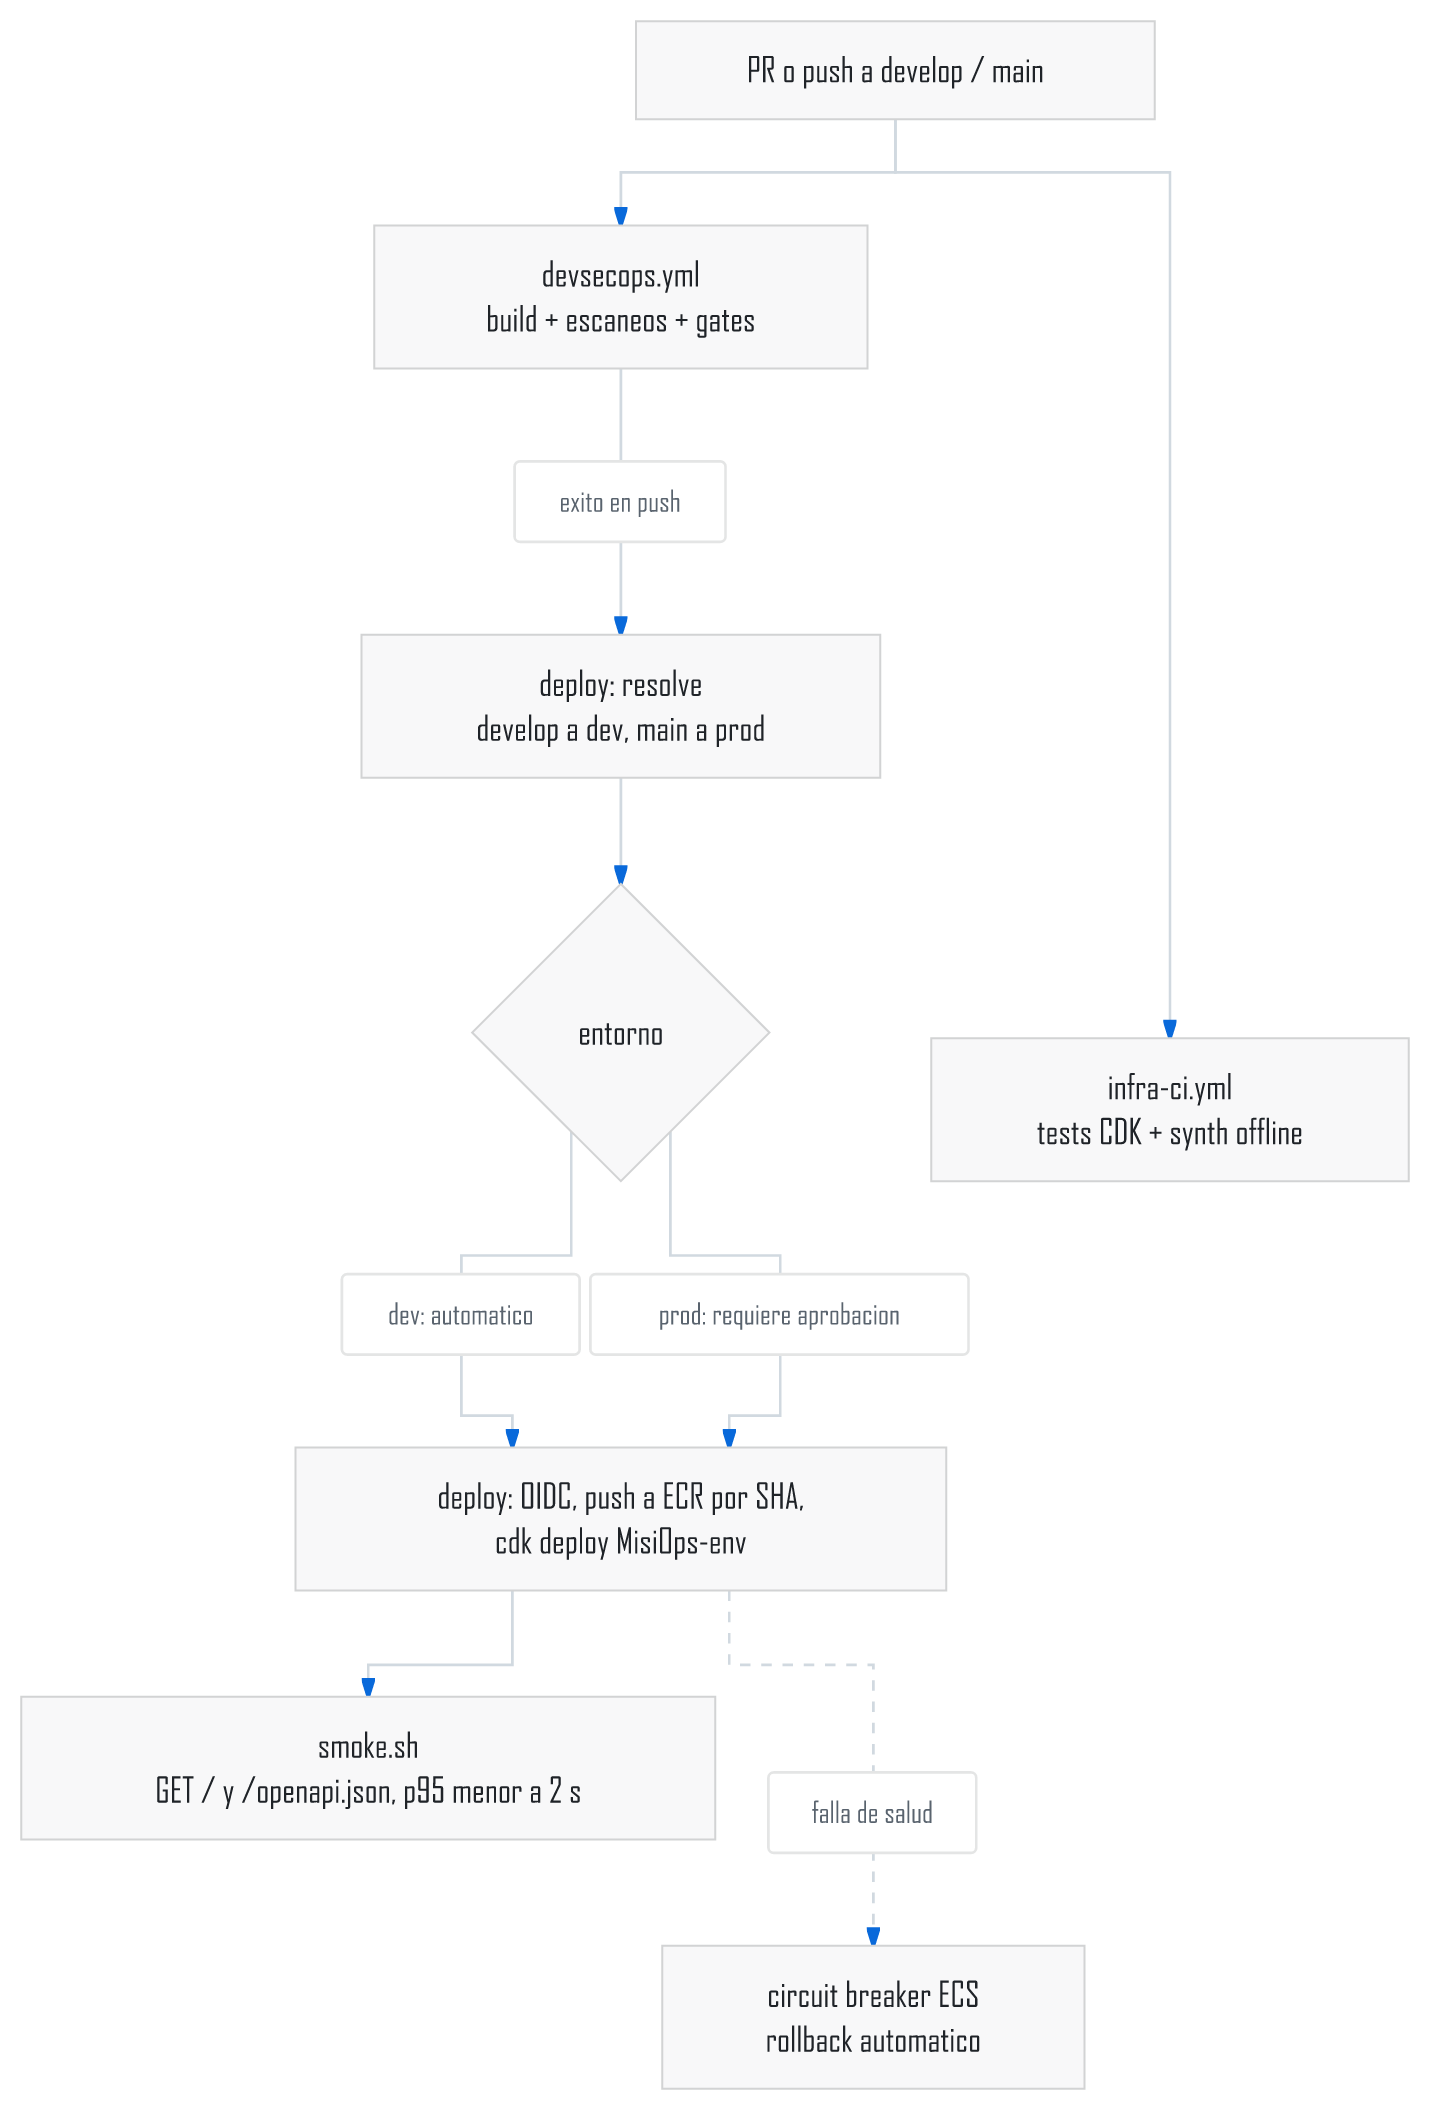
\includegraphics[width=0.55\textwidth]{figures/iac/iac-pipeline.png}
    \caption{Flujo de CI/CD de la infraestructura y del despliegue}
    \label{fig:iac-pipeline}
\end{figure}

\begin{enumerate}
    \item \textbf{\texttt{infra-ci.yml}} corre en cada PR o push a \texttt{develop} que toque \texttt{infra/}. Ejecuta los tests del CDK y un \textit{synth} sin credenciales de \texttt{dev} y \texttt{prod}, y comprueba que la plantilla no contenga ningún \texttt{SecretString}.
    \item \textbf{\texttt{devsecops.yml}} construye una sola vez las imágenes \texttt{linux/arm64}, las escanea y las guarda como artefacto (sección anterior).
    \item \textbf{\texttt{deploy.yml}} (Anexo~\ref{anx:deploy}) se dispara con \texttt{workflow\_run} cuando \texttt{devsecops} termina. Su job \texttt{resolve} solo continúa si la corrida fue un \textbf{push exitoso} y asigna \texttt{develop} $\rightarrow$ \texttt{dev} y \texttt{main} $\rightarrow$ \texttt{prod}. Los PR y las ejecuciones manuales nunca despliegan.
    \item El job \texttt{deploy} corre dentro del GitHub Environment correspondiente: \texttt{dev} es automático y \texttt{prod} espera la aprobación de un revisor. Después:
          \begin{itemize}
              \item asume el rol por OIDC;
              \item descarga el artefacto de imágenes de esa corrida, sin volver a construirlas;
              \item las sube a ECR con el SHA del commit;
              \item ejecuta \texttt{cdk deploy MisiOps-\textless env\textgreater};
              \item corre \texttt{infra/scripts/smoke.sh} contra la URL pública.
          \end{itemize}
    \item El resumen de la corrida registra entorno, commit, digest de ambas imágenes, URL pública, resultado del smoke test y duración. Los despliegues al mismo entorno se encolan (\texttt{concurrency: deploy-\textless env\textgreater}).
\end{enumerate}

\textbf{Rollback.} Si la nueva tarea no pasa el \textit{health check} del balanceador, el \textit{circuit breaker} de ECS vuelve a la definición de tarea anterior, CloudFormation deja el stack en \texttt{UPDATE\_ROLLBACK\_COMPLETE} y la corrida de \texttt{deploy} queda en rojo. Los usuarios siguen atendidos por la versión previa. Para un rollback manual se vuelve a ejecutar \texttt{devsecops} sobre el commit bueno, y eso redespliega esa versión por el mismo camino.

\subsection{Implementación en AWS CloudFormation}

\begin{itemize}
    \item \texttt{infra/bin/misiops.ts} crea la aplicación CDK: el stack \texttt{MisiOps-Foundation} y un \texttt{EnvironmentStack} según el contexto \texttt{-c env=dev|prod}.
    \item \texttt{infra/lib/environment-stack.ts} (unas 230 líneas) declara todos los recursos de un entorno. \texttt{infra/lib/config.ts} concentra las únicas diferencias entre \texttt{dev} y \texttt{prod}: la etiqueta ``dev'' visible en la interfaz, la política de borrado de la base de datos y la protección contra borrado.
    \item \texttt{cdk synth} produce las plantillas CloudFormation en \texttt{cdk.out/}; \texttt{cdk deploy} las envía a CloudFormation, que crea o actualiza los recursos y revierte si algo falla.
    \item \textbf{Pruebas}: 24 tests con \texttt{node:test} y \texttt{aws-cdk-lib/assertions} (20 del stack de entorno y 4 del stack Foundation). Verifican, entre otras cosas, la base de datos sin acceso público y cifrada, los secretos inyectados desde Secrets Manager, los tags inmutables en ECR, la condición de confianza OIDC y el \textit{circuit breaker} con rollback. A eso se suma un test en Bash del smoke script con un \texttt{curl} simulado.
\end{itemize}

Para que una misma imagen sirva en ambos entornos se hicieron dos cambios pequeños en la aplicación. El frontend llama a la API por rutas relativas del mismo dominio: el argumento de build \texttt{NEXT\_PUBLIC\_API\_BASE\_URL} vale vacío por defecto. Además muestra un banner y el sufijo ``· dev'' en el título solo cuando el contenedor tiene \texttt{APP\_ENV=dev}.

\subsection{Evidencias}

\textbf{Primer despliegue de \texttt{dev}} (manual, 2026-11-08). El primer intento de \texttt{cdk deploy MisiOps-dev} se revirtió automáticamente a los 14 minutos: el backend arrancó mientras Aurora seguía aprovisionándose y el \textit{circuit breaker} actuó sin dejar recursos huérfanos. Se corrigió haciendo que el servicio dependa de la base de datos. El segundo intento terminó en 9 minutos y el smoke test pasó, con p95 de 0.67 s en \texttt{GET /} y 0.62 s en \texttt{GET /openapi.json} sobre 20 peticiones. También se verificó de punta a punta el registro, el login, la creación de una transacción y su lectura en el resumen, a través de CloudFront y con los datos persistidos en Aurora.

\textbf{Despliegue automático de \texttt{prod}} (corrida \href{https://github.com/jeffreymonjacastro/MisiOps/actions/runs/43147540236}{43147540236}, 2026-11-12):
\begin{itemize}
    \item Se disparó tras la corrida verde de \texttt{devsecops} sobre \texttt{main} (merge del PR \#179, commit \texttt{8b85bc6}) y esperó la aprobación del revisor del entorno \texttt{prod}.
    \item \texttt{cdk deploy MisiOps-prod} creó el stack completo (52 recursos). El job tardó 10 min 31 s.
    \item URL pública: \url{https://dnowsrpw9uokx.cloudfront.net}.
    \item Smoke test: p95 de 0.175 s en \texttt{GET /} y de 0.098 s en \texttt{GET /openapi.json}.
    \item Digests publicados en ECR: backend \texttt{sha256:b3ed679f\ldots}, frontend \texttt{sha256:3cc14352\ldots}.
\end{itemize}

\begin{figure}[H]
    \centering
    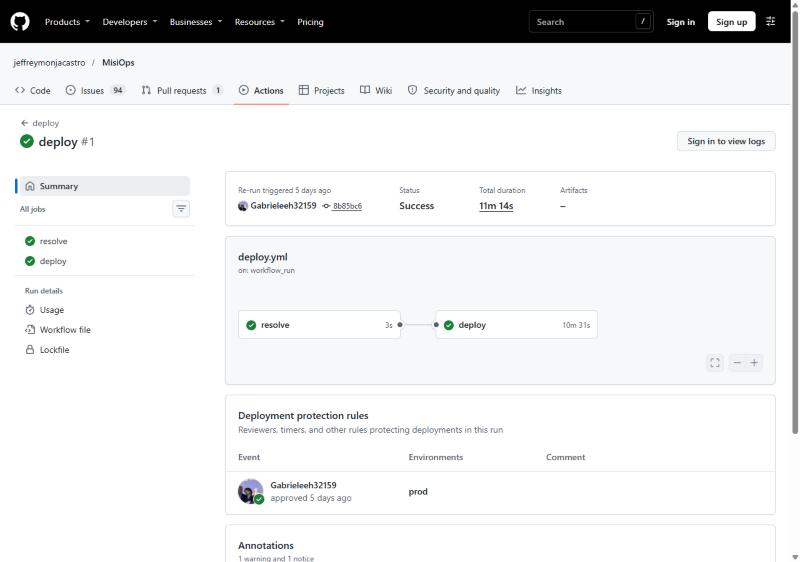
\includegraphics[width=0.9\textwidth]{figures/iac/deploy-run-prod.jpg}
    \caption{Corrida del workflow \texttt{deploy} hacia \texttt{prod}, con la aprobación registrada en las reglas de protección del entorno}
    \label{fig:deploy-prod}
\end{figure}

\begin{figure}[H]
    \centering
    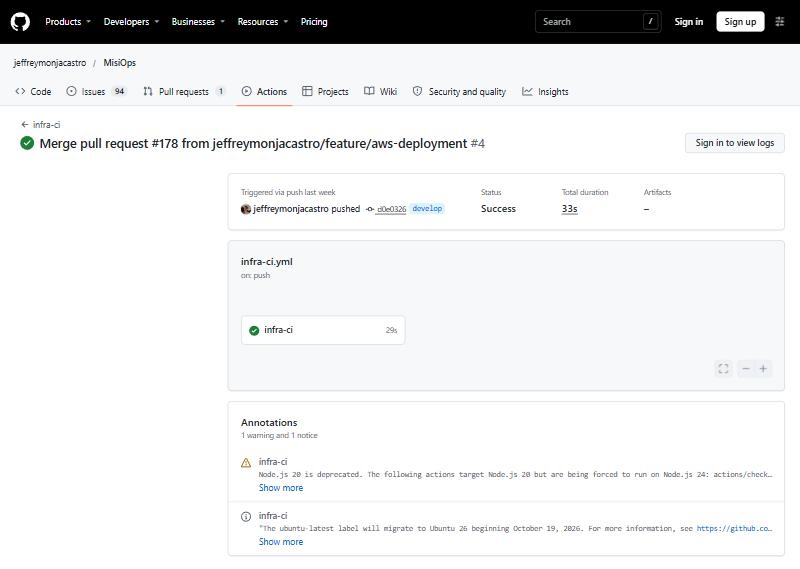
\includegraphics[width=0.9\textwidth]{figures/iac/infra-ci-run.jpg}
    \caption{Corrida de \texttt{infra-ci} (tests del CDK y \textit{synth}) tras el merge del PR \#178 a \texttt{develop}}
    \label{fig:infra-ci}
\end{figure}

\begin{figure}[H]
    \centering
    \begin{minipage}{0.49\textwidth}
        \centering
        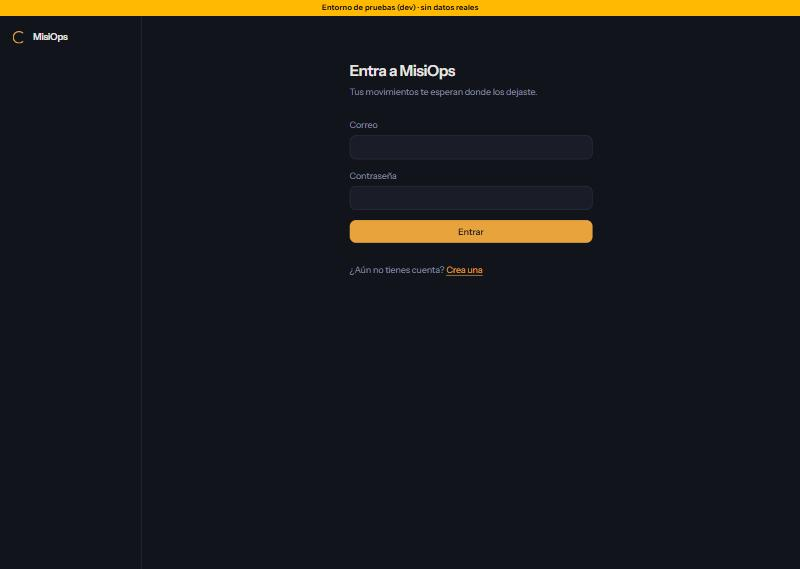
\includegraphics[width=\linewidth]{figures/iac/app-dev.jpg}
        \small (a) \texttt{dev}: \url{https://d2n2ap8z1x33no.cloudfront.net}
    \end{minipage}
    \hfill
    \begin{minipage}{0.49\textwidth}
        \centering
        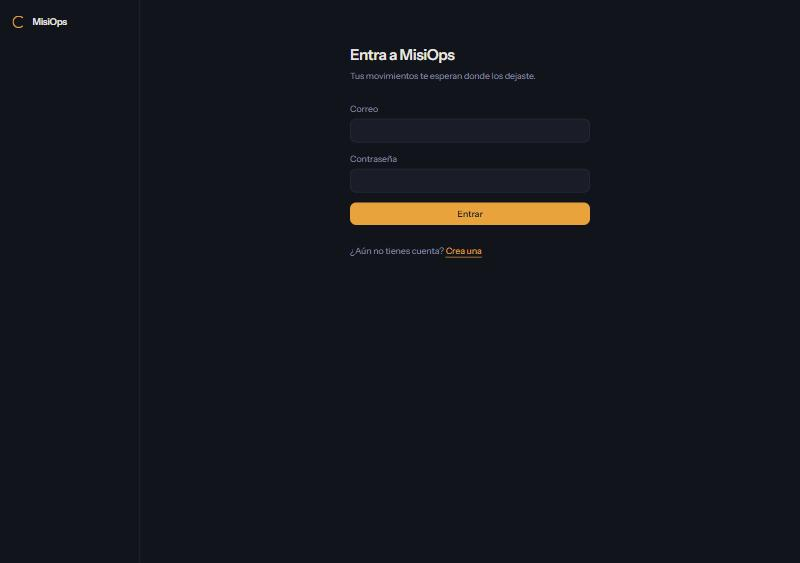
\includegraphics[width=\linewidth]{figures/iac/app-prod.jpg}
        \small (b) \texttt{prod}: \url{https://dnowsrpw9uokx.cloudfront.net}
    \end{minipage}
    \caption{MisiOps desplegado en AWS: \texttt{dev} muestra el banner de entorno de pruebas y \texttt{prod} no}
    \label{fig:apps}
\end{figure}

La guía de operación completa (preparación de la cuenta, aprobación de \texttt{prod}, rollback, logs, costos y destrucción del entorno) está en \texttt{docs/deployment/README.md}.


\section{MLOps}

% NOTA: a la fecha de redacción, el repositorio (develop y main) no contiene código, workflows ni
% capturas de MLOps. Los textos marcados con \pendiente{} deben completarse con la evidencia real.

\subsection{Importancia de MLOps y CRISP-ML(Q)}

Un modelo de machine learning no es un artefacto estático como un binario: su comportamiento depende de los datos con los que se entrenó, y esos datos cambian con el tiempo. MLOps aplica las prácticas de DevOps (versionado, automatización, pruebas, despliegue continuo y monitoreo) a todo el ciclo de vida del modelo: datos, entrenamiento, validación, despliegue y observación en producción. Sin MLOps, los modelos se entrenan a mano en notebooks, no se pueden reproducir, se despliegan sin validar y se degradan sin que nadie lo note (\textit{data drift} o \textit{concept drift}).

CRISP-ML(Q) (\textit{Cross-Industry Standard Process for Machine Learning with Quality assurance}) extiende el clásico CRISP-DM con aseguramiento de calidad en cada fase. Define seis fases iterativas:
\begin{enumerate}
    \item Entendimiento del negocio y de los datos.
    \item Preparación de datos.
    \item Modelado.
    \item Evaluación.
    \item Despliegue.
    \item Monitoreo y mantenimiento.
\end{enumerate}
En cada fase se identifican los riesgos que podrían afectar la calidad del modelo y se definen métodos para mitigarlos. Así cada etapa tiene criterios de salida verificables, lo que encaja con los gates del pipeline ya usados en DevSecOps.

En MisiOps, la constitución del proyecto define como caso de uso de MLOps \textbf{entrenar modelos sobre el historial de transacciones del usuario para predecir su ahorro a fin de mes}. Esa predicción responde directamente al problema de negocio: que el usuario sepa con anticipación si llegará a fin de mes con ahorro o con deuda.

\subsection{Arquitectura de MLOps y componentes}

\pendiente{diagrama de arquitectura de MLOps (\texttt{figures/mlops/arquitectura.png}) y explicación de cada componente: origen de datos, \textit{feature store} o \textit{pipeline} de features, registro de experimentos y modelos, servicio de inferencia y monitoreo.}

\subsection{Pipeline de CI/CD en GitHub Actions}

\pendiente{workflow de MLOps (archivo en \texttt{.github/workflows/}), sus etapas, sus disparadores y una captura de una corrida exitosa.}

\subsection{Implementación}

\subsubsection{Entendimiento del negocio}

El objetivo es estimar, a mitad de mes, el ahorro con el que el usuario cerrará el periodo presupuestario: ingresos menos gastos. Con esa estimación MisiOps podría alertar con anticipación cuando el ritmo de gasto lleve a cerrar el mes en negativo. \pendiente{métrica de éxito del negocio y métrica técnica (por ejemplo, MAE en soles) con su umbral de aceptación.}

\subsubsection{Feature engineering}

\pendiente{origen y volumen de los datos, variables construidas (por ejemplo, gasto acumulado por categoría, ingresos del periodo, días transcurridos, gasto del mismo periodo del mes anterior) y validaciones de calidad de datos.}

\subsubsection{Selección del modelo}

\pendiente{modelos comparados, métricas obtenidas y criterio de selección del modelo final.}

\subsubsection{Smoke test}

\pendiente{prueba automática que valida el modelo empaquetado: carga, predicción sobre un caso conocido y tiempo de respuesta.}

\subsubsection{Despliegue}

\pendiente{forma de servir el modelo (endpoint, contenedor o batch) y relación con la infraestructura de la sección de IaC.}

\subsubsection{Monitoreo}

\pendiente{métricas que se monitorean en producción (deriva de datos, error de predicción, latencia) y criterio para reentrenar.}

\subsection{Evidencias}

\pendiente{capturas de las corridas del pipeline de MLOps, del registro de experimentos o modelos y del modelo desplegado.}


\section{Conclusiones}

\subsection{Lecciones aprendidas}

\textbf{Problema de negocio resuelto.} MisiOps guarda credenciales y datos financieros de sus usuarios. Una fuga o una dependencia vulnerable destruiría la confianza en el producto. Necesitábamos detectar esos riesgos antes de publicar, no después, y poder desplegar de forma repetible y segura.

\textbf{Limitaciones iniciales.} La seguridad dependía de la revisión manual del PR y de \texttt{pip-audit}. No se revisaban secretos en el historial, ni imágenes, ni configuración, ni la aplicación en ejecución. Los resultados quedaban dispersos y nada impedía integrar un cambio inseguro. Además, la aplicación solo corría en local con Docker Compose y no tenía un entorno en la nube.

\textbf{Qué cambió con DevOps.}
\begin{itemize}
    \item La seguridad corre en cada PR, automatizada y con versiones fijadas de cada herramienta.
    \item Los hallazgos llegan a un solo lugar (DefectDojo), con historial y estado de cada uno.
    \item \texttt{main} solo recibe código que pasó todos los escaneos.
    \item La infraestructura es código probado: un merge a \texttt{develop} actualiza \texttt{dev}, y un merge aprobado a \texttt{main} actualiza \texttt{prod} con exactamente las imágenes que se escanearon.
\end{itemize}

\textbf{Ventajas medidas.}
\begin{itemize}
    \item Se cerraron vulnerabilidades críticas reales (Next.js, certifi, imagen de PostgreSQL): los hallazgos críticos activos bajaron de 39 a 3 y los bloqueantes de 263 a 0.
    \item El pipeline de seguridad completo tarda unos 4 minutos, y el despliegue a \texttt{prod} unos 11 minutos incluyendo la aprobación.
    \item El gate demostró su valor en un caso real: además de bloquear el PR de prueba \#131, bloqueó la promoción a \texttt{main} cuando Debian publicó el fix de dos CVE HIGH en la imagen base del backend.
    \item El rollback automático de ECS actuó en el primer despliegue fallido sin dejar recursos huérfanos.
\end{itemize}

\textbf{Lecciones técnicas.}
\begin{itemize}
    \item Un escáner que no alcanza su objetivo no equivale a ``cero hallazgos'': los jobs fallan explícitamente si ZAP no llega a la aplicación.
    \item Un gate útil bloquea solo lo accionable. Bloquear CVE sin fix publicado frenaría todos los merges sin mejorar la seguridad.
    \item Los títulos de \textit{Test} en DefectDojo deben ser únicos por reporte, porque si no una importación cierra los hallazgos de otra.
    \item Construir las imágenes una sola vez y reutilizarlas para escanear, probar y desplegar garantiza que lo que llega a producción es lo que se analizó.
\end{itemize}

\subsection{Recomendaciones}

\begin{itemize}
    \item Alojar DefectDojo en un servidor propio con credenciales robustas, en lugar del equipo local con \texttt{admin/admin} y un túnel ngrok.
    \item Agregar \textit{rate limiting} y bloqueo temporal en \texttt{/auth/login} (amenazas T1 y T10) y rotación de la \texttt{SECRET\_KEY} (T2).
    \item Al vencer la exención EX-001 (2026-12-31), exigir los checks de seguridad también en \texttt{develop}.
    \item Fijar las GitHub Actions por SHA y activar Dependabot o Renovate para actualizar dependencias de forma continua.
    \item Agregar una bitácora de auditoría de los cambios financieros (amenaza T6).
    \item Restringir la política del rol de ejecución de CloudFormation creado por el \textit{bootstrap} de CDK, que hoy conserva \texttt{AdministratorAccess}.
    \item Migrar la CSP del frontend a una política con \textit{nonce} para eliminar \texttt{'unsafe-inline'}.
\end{itemize}


\nocite{*}
\bibliographystyle{plain}
\bibliography{references}

\appendix
\section{Anexos: scripts y configuración}
\label{anx:devsecops-config}

Copia de los archivos del repositorio \url{https://github.com/jeffreymonjacastro/MisiOps} (rama \texttt{develop}) citados en el informe.

\subsection{Workflow \texttt{.github/workflows/devsecops.yml}}
\label{anx:devsecops}

\begin{lstlisting}
name: devsecops

# Security pipeline (specs/011-devsecops). Gates block pull requests into main and pushes to main;
# into develop they only report (constitution exemption EX-001). Jobs and gates:
# specs/011-devsecops/contracts/pipeline-jobs.md

on:
  pull_request:
    branches: [develop, main]
  push:
    branches: [develop, main]
  workflow_dispatch:

permissions:
  contents: read

concurrency:
  group: devsecops-${{ github.ref }}
  cancel-in-progress: true

env:
  ENFORCE: ${{ github.base_ref == 'main' || github.ref == 'refs/heads/main' }}
  SEMGREP_IMAGE: semgrep/semgrep:1.183.0
  GITLEAKS_IMAGE: zricethezav/gitleaks:v8.30.1
  TRUFFLEHOG_IMAGE: trufflesecurity/trufflehog:3.99.8
  TRIVY_IMAGE: aquasec/trivy:0.76.1
  ZAP_IMAGE: ghcr.io/zaproxy/zaproxy:2.17.0

jobs:
  build:
    runs-on: ubuntu-24.04-arm  # linux/arm64 images for Fargate Graviton (specs/012-aws-deployment R2)
    steps:
      - uses: actions/checkout@v4
      - name: Build images once (scanned, attacked and delivered as the same bytes)
        run: |
          docker build -t misiops-backend:latest backend
          docker build -t misiops-frontend:latest frontend
          docker save misiops-backend:latest -o backend.tar
          docker save misiops-frontend:latest -o frontend.tar
      - uses: actions/upload-artifact@v4
        with:
          name: images
          path: "*.tar"
          retention-days: 1

  sast:
    runs-on: ubuntu-latest
    steps:
      - uses: actions/checkout@v4
      - name: Semgrep (backend + frontend source)
        run: |
          mkdir -p reports
          docker run --rm -u "$(id -u):$(id -g)" -e HOME=/tmp -v "$PWD:/src" -w /src "$SEMGREP_IMAGE" \
            semgrep scan --config p/default --config p/python --config p/typescript --metrics=off \
            --json-output reports/semgrep.json --text-output reports/semgrep.txt backend frontend
      - uses: actions/upload-artifact@v4
        if: always()
        with:
          name: report-sast
          path: reports/
          retention-days: 7
      - name: Gate (Semgrep ERROR)
        run: security/scripts/gate.sh Semgrep "$(jq '[.results[] | select(.extra.severity == "ERROR")] | length' reports/semgrep.json)"

  secrets:
    runs-on: ubuntu-latest
    steps:
      - uses: actions/checkout@v4
        with:
          fetch-depth: 0
      - name: Gitleaks (full history)
        run: |
          mkdir -p reports
          docker run --rm -u "$(id -u):$(id -g)" -v "$PWD:/repo" -w /repo "$GITLEAKS_IMAGE" \
            git --config .gitleaks.toml --redact --exit-code 0 \
            --report-format json --report-path reports/gitleaks.json .
      - name: TruffleHog (full history)
        run: |
          docker run --rm -u "$(id -u):$(id -g)" -e HOME=/tmp -v "$PWD:/repo" "$TRUFFLEHOG_IMAGE" \
            git file:///repo --json --no-update --exclude-paths=/repo/security/trufflehog-exclude.txt > reports/trufflehog.json
      - uses: actions/upload-artifact@v4
        if: always()
        with:
          name: report-secrets
          path: reports/
          retention-days: 7
      - name: Gate (any secret)
        run: |
          security/scripts/gate.sh Gitleaks "$(jq length reports/gitleaks.json)"
          security/scripts/gate.sh TruffleHog "$(grep -c '"SourceMetadata"' reports/trufflehog.json || true)"

  sca:
    runs-on: ubuntu-latest
    steps:
      - uses: actions/checkout@v4
      - name: Trivy DB cache key
        id: day
        run: echo "date=$(date -u +%F)" >> "$GITHUB_OUTPUT"
      - uses: actions/cache@v4
        with:
          path: ~/.cache/trivy
          key: trivy-db-${{ steps.day.outputs.date }}
          restore-keys: trivy-db-
      - name: Trivy dependencies (uv.lock, pnpm-lock.yaml) + SBOM
        run: |
          mkdir -p reports ~/.cache/trivy
          trivy() { docker run --rm -u "$(id -u):$(id -g)" -e TRIVY_CACHE_DIR=/cache -v "$HOME/.cache/trivy:/cache" -v "$PWD:/src" -w /src "$TRIVY_IMAGE" "$@"; }
          # docs/ holds archived reports (incl. an SBOM), not project dependencies.
          trivy fs --scanners vuln --skip-dirs docs --ignorefile .trivyignore.yaml --format json --output reports/trivy-deps.json .
          trivy fs --scanners vuln --skip-dirs docs --ignorefile .trivyignore.yaml --skip-db-update --format table --output reports/trivy-deps.txt .
          trivy fs --skip-dirs docs --skip-db-update --format cyclonedx --output reports/sbom.cdx.json .
      - uses: actions/upload-artifact@v4
        if: always()
        with:
          name: report-sca
          path: reports/
          retention-days: 7
      - name: Gate (fixable HIGH/CRITICAL)
        run: security/scripts/gate.sh "Trivy dependencies" "$(jq -f security/scripts/trivy-blocking.jq reports/trivy-deps.json)"

  container:
    needs: build
    runs-on: ubuntu-latest
    steps:
      - uses: actions/checkout@v4
      - uses: actions/download-artifact@v4
        with:
          name: images
      - name: Trivy DB cache key
        id: day
        run: echo "date=$(date -u +%F)" >> "$GITHUB_OUTPUT"
      - uses: actions/cache@v4
        with:
          path: ~/.cache/trivy
          key: trivy-db-${{ steps.day.outputs.date }}
          restore-keys: trivy-db-
      - name: Trivy images (backend, frontend, postgres)
        run: |
          mkdir -p reports ~/.cache/trivy
          trivy() { docker run --rm -u "$(id -u):$(id -g)" -e TRIVY_CACHE_DIR=/cache -v "$HOME/.cache/trivy:/cache" -v "$PWD:/src" -w /src "$TRIVY_IMAGE" "$@"; }
          postgres=$(grep -oE 'image: postgres[^[:space:]]*' docker/docker-compose.yaml | cut -d' ' -f2)
          trivy image --ignorefile .trivyignore.yaml --input backend.tar --format json --output reports/trivy-image-backend.json
          trivy image --ignorefile .trivyignore.yaml --skip-db-update --input frontend.tar --format json --output reports/trivy-image-frontend.json
          trivy image --ignorefile .trivyignore.yaml --skip-db-update --format json --output reports/trivy-image-postgres.json "$postgres"
      - uses: actions/upload-artifact@v4
        if: always()
        with:
          name: report-container
          path: reports/
          retention-days: 7
      - name: Gate (fixable HIGH/CRITICAL, secrets)
        run: |
          rc=0
          for image in backend frontend postgres; do
            security/scripts/gate.sh "Trivy image $image" "$(jq -f security/scripts/trivy-blocking.jq "reports/trivy-image-$image.json")" || rc=1
          done
          exit $rc

  iac:
    runs-on: ubuntu-latest
    steps:
      - uses: actions/checkout@v4
      - name: Trivy config (Dockerfiles) + Semgrep (docker-compose)
        run: |
          mkdir -p reports
          docker run --rm -u "$(id -u):$(id -g)" -e TRIVY_CACHE_DIR=/tmp/trivy -v "$PWD:/src" -w /src "$TRIVY_IMAGE" \
            config --skip-dirs docs --format json --output reports/trivy-config.json .
          # Trivy has no Compose scanner, so the orchestration file goes through Semgrep's compose rules.
          docker run --rm -u "$(id -u):$(id -g)" -e HOME=/tmp -v "$PWD:/src" -w /src "$SEMGREP_IMAGE" \
            semgrep scan --config p/docker-compose --metrics=off --json-output reports/semgrep-compose.json docker
      - uses: actions/upload-artifact@v4
        if: always()
        with:
          name: report-iac
          path: reports/
          retention-days: 7
      - name: Gate (HIGH/CRITICAL misconfigurations)
        run: |
          rc=0
          security/scripts/gate.sh "Trivy config" "$(jq -f security/scripts/trivy-blocking.jq reports/trivy-config.json)" || rc=1
          security/scripts/gate.sh "Semgrep compose" "$(jq '[.results[] | select(.extra.severity == "ERROR")] | length' reports/semgrep-compose.json)" || rc=1
          exit $rc

  dast:
    needs: build
    runs-on: ubuntu-24.04-arm  # linux/arm64 images for Fargate Graviton (specs/012-aws-deployment R2)
    steps:
      - uses: actions/checkout@v4
      - uses: actions/download-artifact@v4
        with:
          name: images
      - name: Start the stack from the scanned images
        run: |
          docker load -i backend.tar && docker load -i frontend.tar
          # Throwaway credentials generated per run; never committed (FR-018).
          pw=$(openssl rand -hex 24)
          printf 'POSTGRES_PASSWORD=%s\nSECRET_KEY=%s\n' "$pw" "$(openssl rand -hex 32)" > docker/.env.dev
          printf '%s' "$pw" > docker/pg_password.txt
          docker compose -f docker/docker-compose.yaml up -d --no-build
          curl -fsS --retry 30 --retry-all-errors --retry-delay 2 -o /dev/null http://localhost:8000/
          curl -fsS --retry 30 --retry-all-errors --retry-delay 2 -o /dev/null http://localhost:3000/
      - name: Get a bearer token for the authenticated API scan
        run: |
          email="zap-${GITHUB_RUN_ID}@example.com" pass=$(openssl rand -hex 16)
          body=$(jq -nc --arg e "$email" --arg p "$pass" '{name: "ZAP scanner", email: $e, password: $p}')
          curl -fsS -X POST http://localhost:8000/api/v1/auth/register -H 'Content-Type: application/json' -d "$body" -o /dev/null
          token=$(curl -fsS -X POST http://localhost:8000/api/v1/auth/login -H 'Content-Type: application/json' -d "$body" | jq -r .access_token)
          echo "::add-mask::$token"
          echo "ZAP_TOKEN=$token" >> "$GITHUB_ENV"
      - name: ZAP baseline (frontend) and API scan (OpenAPI, authenticated)
        run: |
          mkdir -p reports && chmod 777 reports
          cp security/zap/rules.conf reports/zap-rules.conf
          zap() { docker run --rm --network host -v "$PWD/reports:/zap/wrk:rw" "$@"; }
          zap "$ZAP_IMAGE" zap-baseline.py -t http://localhost:3000 -c zap-rules.conf -I \
            -x zap-frontend.xml -r zap-frontend.html -J zap-frontend.json || true
          zap -e ZAP_AUTH_HEADER_VALUE="Bearer $ZAP_TOKEN" -e ZAP_AUTH_HEADER_SITE=localhost:8000 "$ZAP_IMAGE" \
            zap-api-scan.py -t http://localhost:8000/openapi.json -f openapi -c zap-rules.conf -I \
            -x zap-api.xml -r zap-api.html -J zap-api.json -z "-config scanner.maxScanDurationInMins=10" || true
          # A missing report means ZAP never reached the app: fail instead of reporting "no findings".
          test -s reports/zap-frontend.json && test -s reports/zap-api.json
      - uses: actions/upload-artifact@v4
        if: always()
        with:
          name: report-dast
          path: reports/
          retention-days: 7
      - name: Gate (High-risk alerts)
        run: |
          rc=0
          for scan in frontend api; do
            security/scripts/gate.sh "ZAP $scan" "$(jq '[.site[]?.alerts[]? | select(.riskcode == "3")] | length' "reports/zap-$scan.json")" || rc=1
          done
          exit $rc
      - name: Stop the stack
        if: always()
        run: docker compose -f docker/docker-compose.yaml down -v

  scripts-test:
    runs-on: ubuntu-latest
    steps:
      - uses: actions/checkout@v4
      - run: bash security/tests/test_upload_to_defectdojo.sh

  summary:
    needs: [sast, secrets, sca, container, iac, dast]
    if: always()
    runs-on: ubuntu-latest
    steps:
      - uses: actions/download-artifact@v4
        with:
          pattern: report-*
          path: reports
          merge-multiple: true
      - name: Findings by tool and severity
        run: |
          cd reports
          sev() { jq -r "$1" "$2" 2>/dev/null | sort | uniq -c | awk '{printf "%s %s, ", $1, $2}'; }
          trivy='.Results[]? | (.Vulnerabilities[]?, .Misconfigurations[]?) | .Severity'
          {
            echo "## Security findings (mode: $([ "$ENFORCE" = true ] && echo blocking || echo report-only))"
            echo "| Report | Findings by severity |"
            echo "| --- | --- |"
            for f in semgrep.json semgrep-compose.json; do echo "| $f | $(sev '.results[].extra.severity' "$f") |"; done
            echo "| gitleaks.json | $(jq length gitleaks.json 2>/dev/null) secrets |"
            echo "| trufflehog.json | $(grep -c '"SourceMetadata"' trufflehog.json 2>/dev/null) secrets |"
            for f in trivy-*.json; do echo "| $f | $(sev "$trivy" "$f") |"; done
            for f in zap-frontend.json zap-api.json; do echo "| $f | $(sev '.site[]?.alerts[]? | .riskdesc | split(" ")[0]' "$f") |"; done
          } >> "$GITHUB_STEP_SUMMARY"

  defectdojo:
    needs: [sast, secrets, sca, container, iac, dast]
    if: always()
    continue-on-error: true
    runs-on: ubuntu-latest
    env:
      DEFECTDOJO_URL: ${{ secrets.DEFECTDOJO_URL }}
      DEFECTDOJO_TOKEN: ${{ secrets.DEFECTDOJO_TOKEN }}
    steps:
      - uses: actions/checkout@v4
      - uses: actions/download-artifact@v4
        with:
          pattern: report-*
          path: reports
      - name: Import every report (reimport-scan)
        run: |
          if [ -z "$DEFECTDOJO_URL" ]; then
            echo "skipped: no DefectDojo configured (use security/scripts/import_run.sh ${GITHUB_RUN_ID})"
            exit 0
          fi
          security/scripts/import_run.sh reports

  deliver:
    needs: [sast, secrets, sca, container, iac, dast, scripts-test]
    if: github.event_name == 'push' && github.ref == 'refs/heads/main'
    runs-on: ubuntu-latest
    permissions:
      contents: read
      packages: write
    steps:
      - uses: actions/download-artifact@v4
        with:
          name: images
      - name: Publish the scanned images to GHCR
        env:
          GH_TOKEN: ${{ secrets.GITHUB_TOKEN }}
        run: |
          echo "$GH_TOKEN" | docker login ghcr.io -u "${{ github.actor }}" --password-stdin
          for app in backend frontend; do
            docker load -i "$app.tar"
            for tag in "$GITHUB_SHA" latest; do
              docker tag "misiops-$app:latest" "ghcr.io/jeffreymonjacastro/misiops-$app:$tag"
              docker push "ghcr.io/jeffreymonjacastro/misiops-$app:$tag"
            done
          done
\end{lstlisting}

\subsection{Gate por herramienta: \texttt{security/scripts/gate.sh}}
\label{anx:gate}

\begin{lstlisting}
#!/usr/bin/env bash
# Security gate (FR-012). Blocks only when ENFORCE=true (pull requests into main, pushes to main);
# otherwise warns, because merges into develop are report-only under constitution exemption EX-001.
# Usage: gate.sh <tool> <blocking-finding-count>
set -euo pipefail

if [ $# -ne 2 ]; then
  echo "usage: $0 <tool> <count>" >&2
  exit 2
fi
tool=$1 count=$2
mode=report-only
[ "${ENFORCE:-false}" = true ] && mode=blocking
[ -n "${GITHUB_STEP_SUMMARY:-}" ] && echo "- **$tool**: $count blocking findings ($mode)" >> "$GITHUB_STEP_SUMMARY"

if [ "$count" -eq 0 ]; then
  echo "$tool: no blocking findings"
elif [ "$mode" = blocking ]; then
  echo "::error::$tool: $count blocking findings"
  exit 1
else
  echo "::warning::$tool: $count findings would block a merge into main (report-only, constitution EX-001)"
fi
\end{lstlisting}

\subsection{Filtro de Trivy: \texttt{security/scripts/trivy-blocking.jq}}
\label{anx:jq}

\begin{lstlisting}
# Blocking findings in a Trivy JSON report (FR-012): fixable HIGH/CRITICAL vulnerabilities,
# HIGH/CRITICAL misconfigurations and any secret. Unfixed vulnerabilities are reported only.
[
  .Results[]?
  | (.Vulnerabilities[]? | select((.Severity == "HIGH" or .Severity == "CRITICAL") and ((.FixedVersion // "") != ""))),
    (.Misconfigurations[]? | select(.Severity == "HIGH" or .Severity == "CRITICAL")),
    (.Secrets[]?)
] | length
\end{lstlisting}

\subsection{Subida a DefectDojo: \texttt{security/scripts/upload\_to\_defectdojo.sh}}
\label{anx:upload}

\begin{lstlisting}
#!/usr/bin/env bash
# Upload one scan report to DefectDojo through /api/v2/reimport-scan/.
# Contract: specs/011-devsecops/contracts/upload-script.md
# Usage: upload_to_defectdojo.sh <scan_type> <test_title> <report_file>
set -euo pipefail

if [ $# -lt 3 ]; then
  echo "usage: $0 <scan_type> <test_title> <report_file>" >&2
  exit 2
fi
scan_type=$1 test_title=$2 report=$3

# A missing file means the scanner did not run; a zero-finding report is still uploaded
# so close_old_findings can close what an earlier run found.
if [ ! -f "$report" ]; then
  echo "skip: $report not found"
  exit 0
fi
for var in DEFECTDOJO_URL DEFECTDOJO_TOKEN; do
  if [ -z "${!var:-}" ]; then
    echo "missing variable: $var" >&2
    exit 1
  fi
done

tmp=$(mktemp -d)
trap 'rm -rf "$tmp"' EXIT

# TruffleHog writes log lines next to findings; DefectDojo only parses the findings.
if [ "$scan_type" = "Trufflehog Scan" ]; then
  grep '"SourceMetadata"' "$report" > "$tmp/trufflehog.json" || true
  report=$tmp/trufflehog.json
fi

# Header from a file keeps the token off the process list and out of logs.
printf 'Authorization: Token %s\n' "$DEFECTDOJO_TOKEN" > "$tmp/auth"

form=(
  -F "scan_type=$scan_type"
  -F "test_title=$test_title"
  -F "file=@$report"
  -F "product_name=${DEFECTDOJO_PRODUCT:-MisiOps}"
  -F "product_type_name=${DEFECTDOJO_PRODUCT_TYPE:-Aplicaciones Web}"
  -F "engagement_name=${DEFECTDOJO_ENGAGEMENT:-CI - ${GITHUB_HEAD_REF:-${GITHUB_REF_NAME:-local}}}"
  -F "auto_create_context=true"
  -F "close_old_findings=true"
  -F "active=true"
  -F "verified=false"
)
[ -n "${GITHUB_RUN_ID:-}" ] && form+=(-F "build_id=$GITHUB_RUN_ID")
[ -n "${GITHUB_SHA:-}" ] && form+=(-F "commit_hash=$GITHUB_SHA")
[ -n "${GITHUB_REF_NAME:-}" ] && form+=(-F "branch_tag=${GITHUB_HEAD_REF:-$GITHUB_REF_NAME}")

status=$(curl -sS -o "$tmp/body" -w '%{http_code}' -X POST \
  "${DEFECTDOJO_URL%/}/api/v2/reimport-scan/" -H "@$tmp/auth" "${form[@]}")

if [ "$status" = "201" ]; then
  echo "ok: $test_title"
else
  echo "error $status: $(cat "$tmp/body")" >&2
  exit 1
fi
\end{lstlisting}

\subsection{Mapa de reportes y parsers: \texttt{security/scripts/reports.tsv}}
\label{anx:reports}

\begin{lstlisting}
# scan_type    test_title    report file (FR-010, distinct titles: research R7)
Semgrep JSON Report    Semgrep - source    semgrep.json
Gitleaks Scan    Gitleaks - history    gitleaks.json
Trufflehog Scan    TruffleHog - history    trufflehog.json
Trivy Scan    Trivy - dependencies    trivy-deps.json
Trivy Scan    Trivy - image backend    trivy-image-backend.json
Trivy Scan    Trivy - image frontend    trivy-image-frontend.json
Trivy Scan    Trivy - image postgres    trivy-image-postgres.json
Trivy Scan    Trivy - config    trivy-config.json
ZAP Scan    ZAP - frontend baseline    zap-frontend.xml
ZAP Scan    ZAP - API    zap-api.xml
Semgrep JSON Report    Semgrep - compose    semgrep-compose.json
\end{lstlisting}

\subsection{Hooks locales: \texttt{.pre-commit-config.yaml}}
\label{anx:precommit}

\begin{lstlisting}
# Local secret blocking (FR-009). Run by .githooks/pre-commit (core.hooksPath); needs pre-commit 4.7.0 or uv.
repos:
  - repo: https://github.com/gitleaks/gitleaks
    rev: v8.30.1
    hooks:
      - id: gitleaks
  - repo: https://github.com/pre-commit/pre-commit-hooks
    rev: v6.0.0
    hooks:
      - id: detect-private-key
\end{lstlisting}

\subsection{Reglas de ZAP: \texttt{security/zap/rules.conf}}
\label{anx:zap}

\begin{lstlisting}
# ZAP rule overrides: <rule id><TAB><IGNORE|WARN|FAIL><TAB><name>
# The pipeline gate counts High-risk alerts from the JSON report (FR-012), so this file
# only holds suppressions. Every IGNORE line needs a comment above it:
# id: <rule> | justification: <why> | review: <YYYY-MM-DD>   (FR-012b)
\end{lstlisting}

\subsection{Workflow \texttt{.github/workflows/infra-ci.yml}}
\label{anx:infraci}

\begin{lstlisting}
name: infra-ci

# Infrastructure gate (specs/012-aws-deployment, FR-007, NFR-007): tests and an offline synth of the CDK app.
# No AWS credentials: the stacks have no context lookups and the region is fixed in infra/bin/misiops.ts.

on:
  pull_request:
    branches: [develop]
    paths: ["infra/**", ".github/workflows/infra-ci.yml"]
  push:
    branches: [develop]
    paths: ["infra/**", ".github/workflows/infra-ci.yml"]

permissions:
  contents: read

jobs:
  infra-ci:
    runs-on: ubuntu-latest
    timeout-minutes: 5
    defaults:
      run:
        working-directory: infra
    steps:
      - uses: actions/checkout@v4
      - uses: pnpm/action-setup@v4
        with:
          version: 9.6.0
      - uses: actions/setup-node@v4
        with:
          node-version: 20
          cache: pnpm
          cache-dependency-path: infra/pnpm-lock.yaml
      - run: pnpm install --frozen-lockfile
      - name: Unit tests (stack assertions + smoke script)
        run: pnpm test
      - name: Synth dev and prod without credentials
        run: |
          pnpm synth -c env=dev -c imageTag=ci -c alertEmail=ci@example.com --quiet
          pnpm synth -c env=prod -c imageTag=ci -c alertEmail=ci@example.com --quiet
          test "$(grep -c '"SecretString"' cdk.out/MisiOps-dev.template.json)" = 0
\end{lstlisting}

\subsection{Workflow \texttt{.github/workflows/deploy.yml}}
\label{anx:deploy}

\begin{lstlisting}
name: deploy

# Deploys the images scanned by the devsecops run that triggered this workflow (specs/012-aws-deployment).
# develop -> dev (automatic, after the pipeline completes; gates are report-only, EX-001)
# main    -> prod (waits for the required reviewer of the GitHub Environment "prod")
# Contract: specs/012-aws-deployment/contracts/deploy-workflow.md

on:
  workflow_run:
    workflows: [devsecops]
    types: [completed]
    branches: [develop, main]

permissions:
  contents: read
  actions: read
  id-token: write

env:
  AWS_REGION: us-east-1

jobs:
  resolve:
    runs-on: ubuntu-latest
    outputs:
      env: ${{ steps.map.outputs.env }}
      deploy: ${{ steps.map.outputs.deploy }}
      sha: ${{ github.event.workflow_run.head_sha }}
      run_id: ${{ github.event.workflow_run.id }}
    steps:
      - id: map
        env:
          BRANCH: ${{ github.event.workflow_run.head_branch }}
          CONCLUSION: ${{ github.event.workflow_run.conclusion }}
          EVENT: ${{ github.event.workflow_run.event }}
        run: |
          case "$BRANCH" in
            develop) env=dev ;;
            main) env=prod ;;
            *) env= ;;
          esac
          deploy=false
          if [ -n "$env" ] && [ "$CONCLUSION" = success ] && [ "$EVENT" = push ]; then deploy=true; fi
          echo "env=$env" >> "$GITHUB_OUTPUT"
          echo "deploy=$deploy" >> "$GITHUB_OUTPUT"
          echo "branch=$BRANCH conclusion=$CONCLUSION event=$EVENT -> env=${env:-none} deploy=$deploy" | tee -a "$GITHUB_STEP_SUMMARY"

  deploy:
    needs: resolve
    if: needs.resolve.outputs.deploy == 'true'
    runs-on: ubuntu-latest
    timeout-minutes: 30
    environment: ${{ needs.resolve.outputs.env }}
    concurrency:
      group: deploy-${{ needs.resolve.outputs.env }}
      cancel-in-progress: false
    env:
      ENV_NAME: ${{ needs.resolve.outputs.env }}
      SHA: ${{ needs.resolve.outputs.sha }}
    steps:
      - name: Start timer
        run: echo "START=$(date +%s)" >> "$GITHUB_ENV"

      - uses: actions/checkout@v4
        with:
          ref: ${{ needs.resolve.outputs.sha }}

      - name: Download the scanned images of the triggering devsecops run (FR-009)
        uses: actions/download-artifact@v8
        with:
          name: images
          run-id: ${{ needs.resolve.outputs.run_id }}
          github-token: ${{ secrets.GITHUB_TOKEN }}
          path: images

      - name: Assume the deploy role through OIDC (FR-011)
        uses: aws-actions/configure-aws-credentials@v6.3.0
        with:
          role-to-assume: ${{ vars.AWS_DEPLOY_ROLE_ARN }}
          aws-region: ${{ env.AWS_REGION }}

      - id: ecr
        uses: aws-actions/amazon-ecr-login@v2

      - name: Push the images to ECR tagged with the commit SHA
        id: push
        env:
          REGISTRY: ${{ steps.ecr.outputs.registry }}
        run: |
          set -euo pipefail
          for app in backend frontend; do
            docker load -i "images/$app.tar"
            docker tag "misiops-$app:latest" "$REGISTRY/misiops-$app:$SHA"
            docker push "$REGISTRY/misiops-$app:$SHA"
            digest=$(docker inspect --format '{{index .RepoDigests 0}}' "$REGISTRY/misiops-$app:$SHA" | cut -d@ -f2)
            echo "${app}_digest=$digest" >> "$GITHUB_OUTPUT"
          done

      - uses: pnpm/action-setup@v4
        with:
          version: 9.6.0
      - uses: actions/setup-node@v4
        with:
          node-version: 20
          cache: pnpm
          cache-dependency-path: infra/pnpm-lock.yaml
      - run: pnpm install --frozen-lockfile
        working-directory: infra

      - name: cdk deploy MisiOps-${{ needs.resolve.outputs.env }}
        working-directory: infra
        run: |
          pnpm cdk deploy "MisiOps-$ENV_NAME" \
            -c "env=$ENV_NAME" -c "imageTag=$SHA" -c "alertEmail=${{ vars.ALERT_EMAIL }}" \
            --require-approval never --outputs-file outputs.json
          echo "PUBLIC_URL=$(jq -r ".\"MisiOps-$ENV_NAME\".PublicUrl" outputs.json)" >> "$GITHUB_ENV"

      - name: Smoke test (FR-017, NFR-009)
        id: smoke
        run: bash infra/scripts/smoke.sh "$PUBLIC_URL" | tee smoke.log

      - name: Summary
        if: always()
        env:
          BACKEND_DIGEST: ${{ steps.push.outputs.backend_digest }}
          FRONTEND_DIGEST: ${{ steps.push.outputs.frontend_digest }}
          SMOKE: ${{ steps.smoke.outcome }}
        run: |
          minutes=$(( ($(date +%s) - START) / 60 ))
          {
            echo "## Deployment to \`$ENV_NAME\`"
            echo "- commit: \`$SHA\` (devsecops run ${{ needs.resolve.outputs.run_id }})"
            echo "- backend digest: \`${BACKEND_DIGEST:-n/a}\`"
            echo "- frontend digest: \`${FRONTEND_DIGEST:-n/a}\`"
            echo "- public URL: ${PUBLIC_URL:-n/a}"
            echo "- smoke test: $SMOKE"
            echo "- duration: ${minutes} min (target: 15 min for updates, 30 min for the first creation)"
          } >> "$GITHUB_STEP_SUMMARY"
\end{lstlisting}

\subsection{Smoke test del despliegue: \texttt{infra/scripts/smoke.sh}}
\label{anx:smoke}

\begin{lstlisting}
#!/usr/bin/env bash
# Post-deployment verification (FR-017, NFR-009, SC-009): the public address serves the web app and the API,
# and both answer within 2 s at p95 over 20 sequential requests. Exit 0 when every check passes, 1 otherwise.
# usage: smoke.sh <public-url>
set -euo pipefail

url=${1:-}
if [ -z "$url" ]; then echo "usage: $0 <public-url>" >&2; exit 2; fi
url=${url%/}
samples=20
p95_limit=2.0
body=$(mktemp); trap 'rm -f "$body"' EXIT

fail() { echo "FAIL - $*"; exit 1; }
# Prints "<status> <seconds>"; a transport error (DNS, TLS, timeout) counts as status 000.
probe() { curl -s -o "$body" -w '%{http_code} %{time_total}' --max-time 10 "$1" || echo "000 10"; }

content_check() { # path expected-substring
  local result status
  result=$(probe "$url$1"); status=${result%% *}
  [ "$status" = "200" ] || fail "GET $1 returned HTTP $status (expected 200)"
  grep -q -- "$2" "$body" || fail "GET $1 body does not contain $2"
  echo "ok   - GET $1 is 200 and contains $2"
}
latency_check() { # path
  local times=() result status
  for _ in $(seq "$samples"); do
    result=$(probe "$url$1"); status=${result%% *}
    [ "$status" = "200" ] || fail "GET $1 returned HTTP $status during sampling"
    times+=("${result#* }")
  done
  [ "${#times[@]}" -eq "$samples" ] || fail "collected ${#times[@]} samples for $1 (expected $samples)"
  local p95
  p95=$(printf '%s\n' "${times[@]}" | sort -g | sed -n "$((samples * 95 / 100))p")
  if awk -v p="$p95" -v l="$p95_limit" 'BEGIN { exit !(p > l) }'; then
    fail "GET $1 p95 ${p95}s over $samples requests exceeds ${p95_limit}s"
  fi
  echo "ok   - GET $1 p95 ${p95}s over $samples requests"
}

content_check / MisiOps
content_check /openapi.json '"openapi"'
latency_check /
latency_check /openapi.json
echo "smoke: all checks passed for $url"
\end{lstlisting}


\end{document}
